
% \section{Введение}


\chapter{Метод оценки синхронизации с произвольными фазовыми задержками.}~\label{chapt2}
\section{Протечка сигнала и ее удаление ортогональным проецированием.}\label{sect1_1}

% Мы можем сделать \textbf{жирный текст} и \textit{курсив}.

Рассмотрим типичную постановку эксперимента в ЭЭГ/МЭГ парадигме.
Пусть, было записано $K$ эпох гомогенной электрофизической
активности продолжительностью $\Delta t$ с помощью энцефалографа (магнитного или электрического),
имеющего $m$ сенсоров.
Далее, допустим, что имеется информация об анатомии мозга испытуемого (этого достаточно
использовать стандартную анатомическую модель мозга,
но для приложений предпочтительнее иметь индивидуальный МРТ снимок).
Последнее допущение позволяет нам рассмотреть пространство источников --- сетку,
состоящую из $n$ точек на коре и аппроксимирующую поверхность мозга испытуемого (\ref{fig:src_space}).
Решая так называемую прямую задачу [2], мы можем осуществить отображение $n$ точек пространства
источников в $m$-мерное пространство сенсоров с оператором отображения $\mathbf{G}$, имея в виду, что
обычно $n \gg m$, так как для качественной аппроксимации нам нужно намного
больше точек на поверхности мозга, чем сенсоров, регистрирующих мозговую активность.

Оператор $\mathbf{G}$ --- суть, решение уравнений Максвелла для точечных источников электромагнитной активности,
расположенных в каждом узле сетки, определяющей конфигурацию источников,
и так как уравнения Максвелла линейны, оператор $\mathbf{G}$ также является линейным~\cite{Hamalainen1993}.
Мы также должны учесть влияние шума источники которого располагаются во внешней среде
и который в первом приближении предполагается белым.

В этих предположениях можем записать порождающую модель данных на сенсорах:

\begin{figure}
\centering
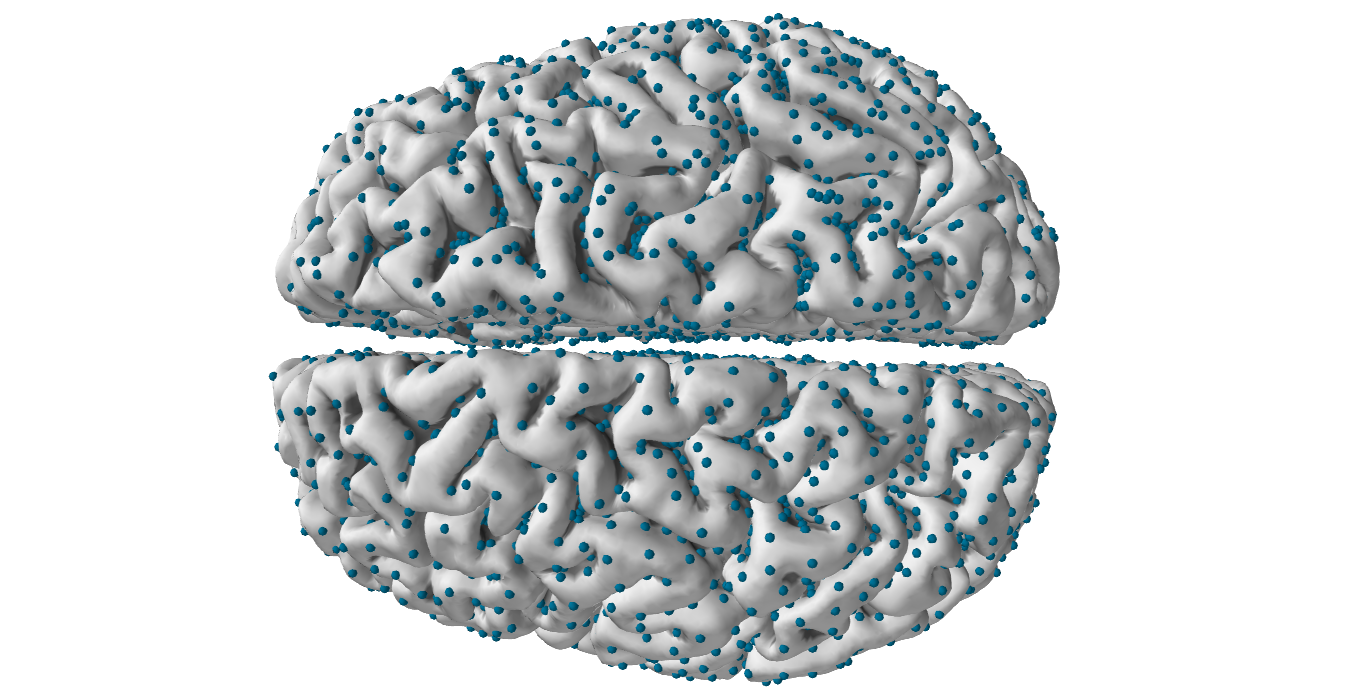
\includegraphics[scale=0.3]{../images/brain.png}
\caption{Пример сетки в пространстве источников,
          построенной на основе трехмерной анатомической модели}\label{fig:src_space}
\end{figure}

\begin{equation}
    \mathbf{x}_k(t) = \mathbf{G} \cdot \mathbf{s}_k(t) + \mathbf{\omega}_k(t),
    \label{gm_ts}
\end{equation}
где $\mathbf{s}_k(t)$ --- $n$-мерный вектор-столбец активаций источников,
$\mathbf{x}_k(t)$ --- $m$-мерный вектор-столбец сигналов на сенсорах,
$t$ --- время, а $\mathbf{G}$ --- $m \times n$ матрица линейного отображения
пространства источников в пространство сенсоров.
Индекс $k$ обозначает номер эпохи.
Применим к (\ref{gm_ts}) частотное преобразование. Существует много способов произвести
эту операцию, например, --- вейвлет-преобразование или узкополосная фильтрация
с последующим аналитическим представлением сигнала.
Мы не будем углубляться в детали теории частотно-временных преобразований;
для подробного изложения предмета см.~\cite{Oppenheim1998},
о применении  частотно-временных преобразований к обработке
электрофизиологических данных см.~\cite{Freeman}.
Мы только упомянем, что вне зависимости от особенностей выбранного
метода образом частотно-временного преобразования матрицы $\mathbf{X}$ размера $m \times T$
будет комплексный тензор, каждый временной срез которого содержит в себе информацию
о фазовом и амплитудном спектре сигнала в каждый момент времени.
Чтобы упростить вывод, мы зафиксируем одну частоту имея в виду,
что дальнейшие выкладки справедливы и для остальных частот преобразования. В итоге мы можем записать:

\begin{equation}
    \hat{\mathbf{x}}_{k,f_i}(t) = \mathbf{G} \cdot \hat{\mathbf{s}}_{k,f_i}(t) + \hat{\mathbf{\omega}}_{k,f_i}(t),
    \label{gm_timefreq}
\end{equation}
где $\hat{\mathbf{x}}, \hat{\mathbf{s}}, \hat{\mathbf{\omega}}$ --- комплекснозначные образы $\mathbf{x}, \mathbf{s}, \mathbf{\omega}$ соответственно.
Для простоты далее будем опускать нижний индекс $f_i$:

\begin{equation}
    \hat{\mathbf{x}}_k(t) = \mathbf{G} \cdot \hat{\mathbf{s}}_k(t) + \hat{\mathbf{\omega}}_k(t)
    \label{gm_timefreq_no_fi}
\end{equation}

\subsection{Порождающая модель матрицы кросс-спектральной плотности и метод ImCoh}\label{sec:imcoh}
Теперь, если мы для каждой эпохи умножим $\hat{\mathbf{x}}_k(t)$ на его эрмитово сопряжение и усредним результат,
мы получим порождающую модель кросс-спектра на сенсорах:

\begin{gather}
           \langle{\hat{\mathbf{x}}_k(t) \hat{\mathbf{x}}_k(t)^{\dag}} \rangle_{k=1}^K =
           \langle{(\mathbf{G} \cdot\hat{\mathbf{s}}_k(t) + \hat{\mathbf{\omega}}_k(t))
                                       (\mathbf{G} \cdot\hat{\mathbf{s}}_k(t) + \hat{\mathbf{\omega}}_k(t))^{\dag}}\rangle_{k=1}^K=\nonumber\\
= \mathbf{G}  \cdot \langle{\hat{\mathbf{s     }}_k(t) \hat{\mathbf{s     }}_k(t)^{\dag}} \rangle_{k=1}^K \cdot \mathbf{G}^T +
   \mathbf{G} \cdot \langle{\hat{\mathbf{s     }}_k(t) \hat{\mathbf{\omega}}_k(t)^{\dag}} \rangle_{k=1}^K + \nonumber\\
        +  \langle{\hat{\mathbf{\omega}}_k(t) \hat{\mathbf{s     }}_k(t)^{\dag}} \rangle_{k=1}^K \cdot \mathbf{G}^T +
           \langle{\hat{\mathbf{\omega}}_k(t) \hat{\mathbf{\omega}}_k(t)^{\dag}} \rangle_{k=1}^K,
    \label{gm_cp_ini}
\end{gather}
\\
где оператор $\langle \cdot \rangle_{k=1}^K$ означает усреднение по эпохам.

Так как шум предполагается белым, а сигнал на сенсорах $\hat{\mathbf{s}}_k$ и шум $\hat{\mathbf{\omega}}_k$ взаимно независимыми,
можем заметить, что второй и третий члены уравнения (\ref{gm_cp_ini}) равны нулю, когда число эпох достаточно велико.
Также отметим, что
$\hat{\mathbf{x     }}_k(t) \hat{\mathbf{x     }}_k(t)^{\dag}$,
$\hat{\mathbf{s     }}_k(t) \hat{\mathbf{s     }}_k(t)^{\dag}$ и
$\hat{\mathbf{\omega}}_k(t) \hat{\mathbf{\omega}}_k(t)^{\dag}$
представляют собой внешние произведения комплексно-значных векторов на свои комплексные сопряжения,
и следовательно являются эрмитовыми матрицами, что означает,
что значения, находящиеся на диагоналях этих матриц, принадлежат к области вещественных чисел.
Это свойство, очевидно, сохраняется и после усреднения.
Более того, раз элементы векторов являются комплексными числами, они могут быть представлены в виде
$\hat{\xi}(t) = r(t)\cdot e^{i\phi(t)}$, где $\phi(t)$ соответствует мгновенной фазе сигнала,
а $r(t)$ амплитуде. Следовательно,
$\langle \hat{\xi}_p \hat{\xi}_q^* \rangle = \langle r_p r_q e^{i\Delta\phi} \rangle$ или,
если для иллюстрации мы примем, что амплитуды и фазы независимы
(справедливость последнего является предметом разногласий для электрофизиологических данных \cite{Lachaux1999}, \cite{imcoh}),
мы получим, что
$\langle \hat{\xi}_p \hat{\xi}_q^* \rangle = \langle r_p r_q \rangle \langle e^{i\Delta\phi} \rangle$.

Из последнего соотношения можно сделать несколько выводов.
Во-первых, элементы матрицы кросс-спектра представляют собой степень стабильности
разности фаз $\Delta\phi$ по эпохам.
Так, если разность фаз была достаточно равномерно распределена по всему возможному
интервалу принимаемых значений, то среднее $\langle e^{i\Delta\phi} \rangle$
будет приблизительно равно нулю.
С другой стороны, если разность фаз сохраняется от эпохи к эпохе,
результирующий коэффициент будет отличен от нуля,
что соответствует случаю установления коннективности между сигналами.
Во-вторых, если разность фаз мала,
элементы взаимного спектра могут быть близки к ненулевому вещественному числу.

Введем следующее обозначение для матрицы кросс-спектральной плотности:

\begin{equation}
    \Cp{v} \stackrel{def}{=} \langle{\hat{\mathbf{v}}_k(t) \hat{\mathbf{v}}_k(t)^{\dag}}\rangle_{k=1}^K, \\
    \label{cp_def}
\end{equation}
Используя определение (\ref{cp_def}) и опуская нулевые члены, (\ref{gm_cp_ini})
перепишется в виде
\begin{equation}
    \Cp{x}(t) = \mathbf{G} \Cp{s}(t) \mathbf{G}^T + \Cp{\omega}(t)
    \label{gm_cp_matr}
\end{equation}

Теперь рассмотрим более детально диагональ матрицы $\Cp{s}$.
Как уже было сказано, элементы главной диагонали этой матрицы являются вещественными числами
и они представляют собой значения мощностей сигналов пространства источников,
имеющих частоту $f_i$. В структуре порождающей модели отражен тот факт,
что после отображения оператором из пространства источников в пространство сенсоров
с помощью оператора $\mathbf{G}$ эти мощностные члены будут смешаны с истинной коннективностью,
и так как исходная система уравнений была сильно недоопределена (условие $n >> m$),
разделить сигналы не представляется возможным.
Математически, этим и объясняется эффект протечки сигнала.

Чтобы внести дополнительную ясность, представим себе ситуацию,
когда синхронизация между источниками полностью отсутствует,
но при этом некоторые участки мозга активны.
В такой постановке все элементы матрицы $\Cp{s}$, лежащие вне главной диагонали,
будут равны нулю, но для $\Cp{x}$ это выполняться не будет.
Пары сенсоров, расположенные близко к активным участкам мозга,
будут иметь большие кросс-спектральные коэффициенты,
что приведет к ложному обнаружению коннективности между источниками.

В ранее упомянутом методе ImCoh (в настоящее время, вероятно,
наиболее часто используемом для измерения коннективности)
предлагается рассматривать только мнимые части уравнения (\ref{gm_cp_matr}),
что уберегает нас от негативного эффекта протечки сигнала,
но при этом мы также теряем действительную часть <<хорошего>> сигнала, несущую
информацию о фазовой синхронизации.

\subsection{Оператор проецирования от протечки сигнала.}

Для более полного использования информации о фазовой синхронизации, содержащейся в кросс-спектре
мы предлагаем другой подход к устранению эффекта протечки сигнала.
Распишем  произведение матриц $\mathbf{G} \Cp{s} \mathbf{G}^T$ в правой части уравнения (\ref{gm_cp_matr}):

\begin{gather}
    \Cp{x}(t) = \sum\limits_{p=1}^n\sum\limits_{q=1}^n\mathbf{g}_p\mathbf{g}_q^T c_{pq}^{\mathbf{ss}}(t) + \Cp{\omega}(t),
    \label{cp_rhs_expanded}
\end{gather}
где $\mathbf{g}_p$ --- столбец матрицы $\mathbf{G}$, который называют \emph{топографией} источника $p$,
поскольку он определяет, каким образом сигнал, поступающий от источника $p$, будет виден на сенсорах.
Можно заметить, что кросс-спектр на уровне сенсоров представляет собой взвешенную сумму внешних произведений топографий,
взятую с коэффициентами, являющимися элементами кросс-спектра из пространства источников.

\subsection{Произведение Кронекера и векторизация}
Векторизуем уравнение (\ref{cp_rhs_expanded}):

\begin{gather}
    vec(\Cp{x}(t)) = \sum\limits_{p=1}^n\sum\limits_{q=1}^n vec(\mathbf{g}_p\mathbf{g}_q^T) c_{pq}^{\mathbf{ss}}(t) + vec(\Cp{\omega}(t))
    \label{cp_rhs_vec}
\end{gather}

Для упрощения записи будем использовать понятие произведения Кронекера.
Произведением Кронекера матриц $A$ и $B$, имеющих размеры $p\times q$ и $r\times s$ соответственно, называется матрица вида

\begin{equation}
    \mathbf{A} \otimes \mathbf{B} \stackrel{def}{=}
    \begin{bmatrix}
        a_{11} \mathbf{B} & a_{12} \mathbf{B} & \dots & a_{1n} \mathbf{B} \\
        a_{21} \mathbf{B} & a_{22} \mathbf{B} & \dots & a_{2n} \mathbf{B} \\
        \vdots            & \vdots            & \dots & \vdots            \\
        a_{m1} \mathbf{B} & a_{m2} \mathbf{B} & \dots & a_{mn} \mathbf{B}
        \label{kron_def}
     \end{bmatrix}
\end{equation}

Произведение Кронекера является билинейной ассоциативной операцией:

\begin{gather}
     \mathbf{A} \otimes (\mathbf{B} + \mathbf{C}) = \mathbf{A} \otimes \mathbf{B} + \mathbf{A} \otimes \mathbf{C} \\
    (\mathbf{A} + \mathbf{B}) \otimes \mathbf{C} = \mathbf{A} \otimes \mathbf{C} + \mathbf{B} \otimes \mathbf{C} \\
    \alpha(\mathbf{A} \otimes \mathbf{B}) = (\alpha\mathbf{A}) \otimes \mathbf{B} = \mathbf{A} \otimes (\alpha\mathbf{B}) \\
    \mathbf{A} \otimes(\mathbf{B} \otimes \mathbf{C}) =
   (\mathbf{A} \otimes \mathbf{B})\otimes \mathbf{C} =
    \mathbf{A} \otimes \mathbf{B} \otimes \mathbf{C}
\end{gather}

Заметим также, что произведение Кронекера не является симметричным: $\mathbf{A} \otimes \mathbf{B} \neq \mathbf{B} \otimes \mathbf{A}$.
Приведем другие полезные соотношения:

\begin{gather}
    (\mathbf{A} \otimes \mathbf{B})^T = \mathbf{A}^T \otimes \mathbf{B}^T \\
    (\mathbf{A} \otimes \mathbf{B}) (\mathbf{C} \otimes \mathbf{D}) = (\mathbf{A} \mathbf{B}) \otimes (\mathbf{C} \mathbf{D})
\end{gather}

Отметим особенно интересное для нас свойство произведения Кронекера,
связывающее его с процедурой векторизации.  Для матриц $\mathbf{A}$,
$\mathbf{B}$, $\mathbf{C}$ справедливо (доказательство см. в~\cite{neudecker}):

\begin{equation}
    vec(\mathbf{A} \mathbf{B} \mathbf{C}) = (\mathbf{C}^T \otimes \mathbf{A}) vec(\mathbf{B})
    \label{eq:kron_vec}
\end{equation}

В нашем случае приведенное выражение принимает самую простую форму:

\begin{gather}
    vec[\mathbf{g}_p \mathbf{g}_q^T] = vec\left[
        \begin{pmatrix}
            g_p^1 \\
            \vdots \\
            g_p^m
        \end{pmatrix}
    \cdot 1 \cdot
    \begin{pmatrix}
        g_q^1 & \dots & g_q^m
    \end{pmatrix}
    \right] = %\nonumber \\
    \begin{pmatrix}
        g_q^1 \\
        \vdots \\
        g_q^m
    \end{pmatrix}
    \otimes
    \begin{pmatrix}
        g_p^1 \\
        \vdots \\
        g_p^m
    \end{pmatrix}
    \cdot
    vec(1) =
    \mathbf{g}_q \otimes \mathbf{g}_p,
\end{gather}


где $\mathbf{g}_q \otimes \mathbf{g}_p$ представляет собой вектор-столбец размера $m^2 \times 1$.
Введем понятие \emph{коммутационной матрицы}~\cite{neudecker}.
Коммутационная матрица --- это матрица, которая связвает операции транспонирования и векторизации
и определяется следующим соотношением:

\begin{equation}
    vec(\mathbf{A}) = \mathbf{K}^{(m,n)} vec(\mathbf{A}^T)
    \label{eq:commutation_matrix_def}
\end{equation}
где $\mathbf{A}$~--- матрица размером $m \times n$, а матрица $\mathbf{K}^{(m,n)}$ имеет размеры
$mn \times mn$.
Матрица $K^{(m,n)}$ является частным случаем матрицы перестановок и
может быть получена из единичной перестановкой строк.

Далее нас будет интересовать только случай квадратных матриц $\mathbf{A}$.
Получим в явном виде выражение для коммутационной матрицы в случае квадратных матриц.

Пусть матрица $\mathbf{A}$ имеет размеры $n \times n$. Обозначим соответствующую ей коммутационную матрицу
как $\mathbf{K}_n$
Обозначим символом $\mathbf{e}_i$ вектор-столбец длины $n$, у которого на $i$-ом месте стоит
единица, а на всех остальных --- нули. Тогда для векторизации $\mathbf{A}^T$ будем иметь:

\begin{multline}
    vec\left(\mathbf{A}^T\right) = vec\left(\sum_{i,j} A_{i,j} \mathbf{e}_j \mathbf{e}_i^T\right) =
    vec\left(\sum_{i,j} (\mathbf{e}_i^T \mathbf{A} \mathbf{e}_j)(\mathbf{e}_j \mathbf{e}_i^T)\right) = \\
  = vec\left(\sum_{i,j} \mathbf{e}_j \mathbf{e}_i^T \mathbf{A} \mathbf{e}_j\mathbf{e}_i^T\right) =
    \sum_{i,j} vec\left(\mathbf{e}_j \mathbf{e}_i^T \mathbf{A} \mathbf{e}_j \mathbf{e}_i^T\right) =
    \left(\sum_{i,j} (\mathbf{e}_i \mathbf{e}_j^T) \otimes (\mathbf{e}_j \mathbf{e}_i^T) \right)vec(\mathbf{A})
\end{multline}

Таким образом,
\begin{equation}
    \mathbf{K}_n =  \sum_{i,j} (\mathbf{e}_i \mathbf{e}_j^T) \otimes (\mathbf{e}_j \mathbf{e}_i^T)
    \label{eq:commutation_matrix_formula}
\end{equation}

Теперь перепишем выражение (\ref{cp_rhs_vec}), используя новые обозначения:

\begin{equation}
    vec(\Cp{x}(t)) = \sum\limits_{p=1}^n\sum\limits_{q=1}^n
    \mathbf{g}_q\otimes \mathbf{g}_p \cdot c_{pq}^{\mathbf{ss}}(t) + vec(\Cp{\omega}(t))
    \label{cp_rhs_kron}
\end{equation}
Теперь можно видеть, что векторизованный кросс-спектр на уровне сенсоров представлен линейной
комбинацией векторов $\mathbf{g}_q \otimes \mathbf{g}_p$ в $m^2$-мерном векторном пространстве.
Назовем эти векторы \emph{2-топографиями}.
Нам уже известно, что эффект протечки сигнала, от которого необходимо избавиться,
обусловлен 2-топографиями особого вида $\mathbf{g}_p \otimes \mathbf{g}_p$ (всего $n$ векторов),
конкретный вид которых нам задан через оператор $\mathbf{G}$.
Следовательно, мы можем спроецировать выражение (\ref{cp_rhs_kron}) ортогонально линейному пространству,
натянутому на 2-топографии источников протечки сигнала.

\subsection{Построение оператора проецирования}
\label{sec:psiicos_projection}
Прежде чем мы начнем построение оператора ортогональной проекции от подпространства протечки сигнала,
необходимо понять, как соотносится подпространство протечки сигнала с линейными оболочками
2-топографий действительной и мнимой частей порождающей модели кросс-спектра на сенсорах.

Во-первых, выделим в уравнении (\ref{cp_rhs_kron}) действительную и мнимую части.
Заметим, что так как матрица $\Cp{s}$ является эрмитовой,
$c^{\mathbf{ss}}_{pq} = \overline{c^{\mathbf{ss}}_{qp}}$ (верхняя черта обозначает комплексное сопряжение):

\begin{gather}
    \sum\limits_{p=1}^n\sum\limits_{q=1}^n \mathbf{g}_q\otimes \mathbf{g}_p \cdot c_{pq}^{\mathbf{ss}}(t) =
    Re\left(\sum\limits_{p,q=1}^{n,n} \mathbf{g}_q\otimes \mathbf{g}_p \cdot c_{pq}^{\mathbf{ss}}(t)\right) +
     i \cdot Im\left(\sum\limits_{p,q=1}^{n,n}
     \mathbf{g}_q\otimes \mathbf{g}_p \cdot c_{pq}^{\mathbf{ss}}(t)\right) = \nonumber \\
           = \sum\limits_{p\leq q}^{n,n} (\mathbf{g}_q\otimes \mathbf{g}_p + \mathbf{g}_p\otimes \mathbf{g}_q)
           Re\left(c_{pq}^{\mathbf{ss}}(t)\right) +
     i \cdot \sum\limits_{p<q}^{n,n} (\mathbf{g}_q\otimes \mathbf{g}_p - \mathbf{g}_p\otimes \mathbf{g}_q)
           Im\left(c_{pq}^{\mathbf{ss}}(t)\right)
    \label{eq:cp_re_im}
\end{gather}

Отметим изменения в индексах суммирования.

Для удобства обозначим линейное пространство, натянутое на 2-топографии, ответственные за протечку сигнала, как
$S_{SL}$, а линейную оболочку 2-топографий мнимой части --- $S_{Im}$.

Из уравнения (\ref{eq:cp_re_im}) видно, что 2-топографии действительной и мнимой частей устроены по-разному,
а именно, --- векторы $\mathbf{g}_q \otimes \mathbf{g}_p + \mathbf{g}_p \otimes \mathbf{g}_q$
являются симметричными, тогда как 2-топографии мнимых частей
$\mathbf{g}_q \otimes \mathbf{g}_p - \mathbf{g}_p \otimes \mathbf{g}_q$ антисимметричны по индексам $p, q$.
Нас интересует, как это структурное отличие проявляется во взаимосвязи подпространств $S_{Re}$ и $S_{Im}$ с
подпространством протечки сигнала $S_{VC}$.
Покажем, что  2-топографии мнимой части ортогональны векторам,
на которые натянуто подпространство объемной проводимости:
\begin{gather}
    (\mathbf{g}_s \otimes \mathbf{g}_s)^T(\mathbf{g}_q \otimes \mathbf{g}_p - \mathbf{g}_p \otimes \mathbf{g}_q) =
        (\mathbf{g}_s^T \otimes \mathbf{g}_s^T)(\mathbf{g}_q \otimes \mathbf{g}_p) -
        (\mathbf{g}_s^T \otimes \mathbf{g}_s^T)(\mathbf{g}_p \otimes \mathbf{g}_q) = \nonumber \\
       =(\mathbf{g}_s^T \mathbf{g}_q \otimes \mathbf{g}_s^T \mathbf{g}_p -
         \mathbf{g}_s^T \mathbf{g}_p \otimes \mathbf{g}_s^T \mathbf{g}_q) \stackrel{*}{=}
        (\mathbf{g}_s^T \mathbf{g}_p \mathbf{g}_s^T \mathbf{g}_q -
         \mathbf{g}_s^T \mathbf{g}_p \mathbf{g}_s^T \mathbf{g}_q) = 0
         \label{eq:vc_ort_im}
\end{gather}

Равенство $*$ сохраняется, так как $\mathbf{g}^T_s \mathbf{g}_q$ и $\mathbf{g}_s^T \mathbf{g}_p$
являются скалярными величинами, и мы можем опустить операцию ``$\otimes$'' и поменять местами множители.
Из (\ref{eq:vc_ort_im}) можно видеть,
что подпространство объемной проводимости ортогонально мнимой части подпространства.
Для действительной части такое соотношение не сохраняется:
\begin{gather}
    (\mathbf{g}_s \otimes \mathbf{g}_s)^T(\mathbf{g}_q \otimes \mathbf{g}_p + \mathbf{g}_p \otimes \mathbf{g}_q) =
        (\mathbf{g}_s^T \otimes \mathbf{g}_s^T)(\mathbf{g}_q \otimes \mathbf{g}_p) +
        (\mathbf{g}_s^T \otimes \mathbf{g}_s^T)(\mathbf{g}_p \otimes \mathbf{g}_q) = \nonumber \\
       =(\mathbf{g}_s^T \mathbf{g}_q \otimes \mathbf{g}_s^T \mathbf{g}_p +
         \mathbf{g}_s^T \mathbf{g}_p \otimes \mathbf{g}_s^T \mathbf{g}_q) =
        2\langle\mathbf{g}_s, \mathbf{g}_p\rangle \langle\mathbf{g}_s, \mathbf{g}_q\rangle
         \label{eq:vc_ort_re}
\end{gather}

После проведенных операций легко увидеть, что проекция ортогонально подпространству протечки сигнала
оказывает влияние на подпространство действительной части кросс-спектра на источниках.
Следовательно, нужно добиться того, чтобы протечка сигнала была удалена из данных
насколько это возможно с учетом минимального воздействия на подпространство
действительной части кросс-спектра (см.рис.~\ref{fig:subspaces}).
Для достижения этой цели необходимо уменьшить размерность подпространства
объемной проводимости неким оптимальным способом.

\begin{figure}[htbp]
\centering
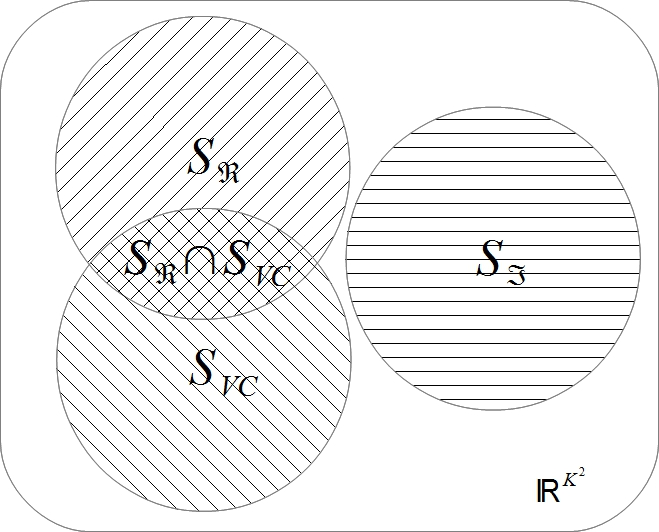
\includegraphics[width=12cm]{./images/SetsReImVC.jpg}
\caption{Взаимосвязь подпространств для кросс-спектра на уровне сенсоров}
\medskip
\small
Подпространство протечки сигнала $S_{SL}$ и подпространство действительной части кросс-спектра $S_{\Re}$
имеют непустое пересечение. Кроме того, оба этих подпространства ортогональны подпространству мнимой
части кросс-спектра $S_{\Im}$.
Пересечение $S_{SL}$ с $S_{\Re}$ содержит вклад как от протечки сигнала,
так и от истинно взаимодействующих источников,
расположенных близко друг к другу и характеризующихся малой разностью фаз.
\label{fig:subspaces}
\end{figure}%
Имея в виду все вышеперечисленное, вернемся к построению проектора.
Рассмотрим матрицу, составленную из вектор-столбцов, образующих подпространство протечки сигнала:

\begin{equation}
    \mathbf{F} =
    \begin{bmatrix}
        |                                 & |                                 &       & |                                 \\
        \mathbf{g}_1 \otimes \mathbf{g}_1 & \mathbf{g}_2 \otimes \mathbf{g}_2 & \dots & \mathbf{g}_n \otimes \mathbf{g}_n \\
        |                                 & |                                 &       & |
    \end{bmatrix}
\end{equation}

Произведем сингулярное разложение матрицы $\mathbf{F}$ \cite{Golub1996}.

\begin{equation}
    \mathbf{F} = \mathbf{USV}^T
    =
    \begin{bmatrix}
        |            & |            &        & |       \\
        \mathbf{u}_1 & \mathbf{u}_2 & \dots  & \mathbf{u}_{m^2} \\
        |            & |            &        & |
    \end{bmatrix}
    % S
    % \begin{pmatrix}
    %   \lambda_1 & 0         & \dots   & 0             & 0 & \dots & 0 \\
    %   0         & \lambda_2 & \dots   & \vdots        & 0 & \dots & 0 \\
    %   \vdots    &           & \ddots  & 0             & 0 & \dots & 0 \\
    %   0         & \dots     & \dots   & \lambda_{m^2} & 0 & \dots & 0
    % \end{pmatrix}
    \begin{pmatrix}
        \lambda_1 & 0         & \dots    \\
        0         & \lambda_2 & \dots    \\
        \vdots    &           & \ddots
    \end{pmatrix}
    % Diag(\lambda_1, \dots, \lambda_{m^2})
    \begin{bmatrix}
        - & \mathbf{v}_1 & - \\
        - & \mathbf{v}_2 & - \\
          & \dots        &   \\
        - & \mathbf{v}_n & -
    \end{bmatrix}
    \label{eq:svd_f_fixed_or}
\end{equation}
\\
В соответствии со свойствами сингулярного разложения, первые $r$ колонок матрицы $\mathbf{U}$
образуют ортонормальный базис $r$-мерного линейного пространства,
являющегося лучшим $r$-мерным приближением $n$-мерного
подпространства протечки сигнала. Используем эти $r$ векторов для построения проектора с уменьшенным рангом:

\begin{gather}
    \mathbf{U}_r =
    \begin{bmatrix}
        |            & |            &        & |       \\
        \mathbf{u}_1 & \mathbf{u}_2 & \dots  & \mathbf{u}_r \\
        |            & |            &        & |
    \end{bmatrix}\label{eq:U_fixed_or};\\
    \mathbf{P}_r = \mathbf{I} - \mathbf{U}_r \mathbf{U}_r^T\label{eq:P_fixed_or}
 \end{gather}

Итак, мы построили оператор проекции ортогонально подпространству протечки сигнала $\mathbf{P}_r$
с сокращенным рангом $r$.
Умножение уравнения (\ref{cp_rhs_kron}) на этот оператор приводит к тому, что  из порождающей
модели кросс-спектра на уровне сенсоров частично удаляются члены ответственные за эффект протечки сигнала;
параметр $r$ при этом определяет баланс между желаемым уровнем очистки от протечки сигнала и
воздействием проектора на действительную часть кросс-спектра.

Окончательно, выражение для кросс-спектра на уровне сенсоров после проекции от протечки сигнала
запишется в виде:

\begin{equation}
    vec(\Cp{x})^\perp = \mathbf{P}_r vec(\Cp{x}) =
    \sum\limits_{p=1}^n\sum\limits_{q=1}^n \mathbf{P}_r \mathbf{g}_q\otimes
    \mathbf{g}_p \cdot c_{pq}^{\mathbf{ss}}(t) + \mathbf{P}_r vec(\Cp{\omega}(t))
    \label{eq:cp_final}
\end{equation}

Или, пользуясь \ref{eq:cp_re_im}:
\begin{multline}
    vec(\Cp{x})^\perp = \sum\limits_{p\leq q}^{n,n}
    \mathbf{P}_r(\mathbf{g}_q\otimes \mathbf{g}_p + \mathbf{g}_p\otimes \mathbf{g}_q)
           Re\left(c_{pq}^{\mathbf{ss}}(t)\right) + \\
    + i \cdot \sum\limits_{p<q}^{n,n} (\mathbf{g}_q\otimes \mathbf{g}_p - \mathbf{g}_p\otimes \mathbf{g}_q)
           Im\left(c_{pq}^{\mathbf{ss}}(t)\right) +
           \mathbf{P}_r vec(\Cp{\omega}(t))
    \label{eq:cp_final_re_im}
\end{multline}

Отметим, что в мнимой части \ref{eq:cp_final_re_im} оператор проецирования $\mathbf{P}_r$ можно опустить
в силу \ref{eq:vc_ort_im}.

Элементы полученного таким образом векторизованного кросс-спектра $vec(\Cp{x})^\perp$ теперь могут быть
использованы для оценки коннективностей как на уровне сенсоров, так и в источниках.

\subsection{Модели со свободной ориентацией диполя}
С точки зрения анатомии каждая топография прямой модели $\mathbf{G}$
представляет собой распределение электромагнитного поля,
порождаемого так называемыми первичными токами, то есть токами,
текущими через апикальные дендриты кортикальных пирамидальных нейронов.
Так как апикальные дендриты расположены перпендикулярно к кортикальной мантии,
первичные токи по отношению к кортикальной мантии также имеют нормальную ориентацию.
Следовательно, точность прямой модели напрямую зависит от точности оценки вектора нормали
к поверхности коры, а значит и от количества точек, используемых для аппроксимации поверхности коры.
Вместе с тем, хотя современное моделирование с использованием метода магнитно-резонансной
томографии позволяет получать весьма детальную реконструкцию мозга с размером аппроксимирующих сеток
порядка нескольких сотен тысяч узлов, использование столь подробных сеток приводит к значительному
ухудшению производительности алгоритмов, работающих в пространстве источников, вследствие высоких затрат
по памяти и вычислительному времени при работе с большими массивами данных.

По этой причине использование разреженных сеток со сравнительно небольшим числом узлов стало
общепринятой практикой. Как уже отмечалось выше, недостаток такого подхода состоит в том, что
при прореживании сетки эффективная ориентация локальной нормали к коре становится неопределенной.

Неопределенность появляется из-за того, что после разрежения размер области на коре, соответствующей отдельно
взятому узлу сетки, возрастает, и так как каждая такая область характеризуется в общем случае
переменной кривизной, эффективная ориентация токового диполя,
находящегося внутри отдельно взятой области аппроксимации,
будет зависеть от того, в какой именно части области находился диполь в тот или иной момент записи.

Частично справиться с этим эффектом позволяют модели, со \emph{свободной ориентацей диполя},
в которых эффективная ориентация становится дополнительным параметром,
который необходимо оценить из данных~\cite{Lin2006}.

Для учета свободной ориентации следует представить топографию в точке $p$ коры в виде линейной
комбинации трех ортогональных друг к другу векторов топографии, размещенных в одной точке:
\begin{equation}
    \mathbf{g}_p = \mathbf{g}_p^x \xi + \mathbf{g}_p^y \eta + \mathbf{g}_p^z \zeta =
    [\mathbf{g}_p^x, \mathbf{g}_p^y, \mathbf{g}_p^z] \left(
    \begin{array}{ccc}
        \xi \\
        \eta \\
        \zeta
    \end{array}
    \right)
    \label{loose_or}
\end{equation}

В случае МЭГ измерений, для модели сферически симметричного проводника,
магнитное поле от токового диполя с радиальной ориентацией равно нулю, и следовательно
введенная тройка векторов может быть заменена парой диполей в плоскости,
перпендикулярной радиальному направлению для каждого узла.
Следовательно, уравнение (\ref{loose_or}) перепишется для МЭГ в виде

\begin{equation}
    \mathbf{g}_p = \mathbf{g}_p^x \xi + \mathbf{g}_p^y \eta = [\mathbf{g}_p^x, \mathbf{g}_p^y] \left(
    \begin{array}{ccc}
        \xi \\
        \eta
    \end{array}
    \right)
    \label{loose_or_meg}
\end{equation}

Соответственно изменятся выражения и для 2-топографий протечки сигнала:

\begin{gather}
    \mathbf{g}_p \otimes \mathbf{g}_p = (\mathbf{g}_p^x \xi
                                      + \mathbf{g}_p^y \eta) \otimes (\mathbf{g}_p^x \xi
                                      + \mathbf{g}_p^y \eta) = \nonumber \\
                                      = \mathbf{g}_p^x \otimes \mathbf{g}_p^x \xi^2
                                      + \mathbf{g}_p^x \otimes \mathbf{g}_p^y \xi \eta
                                      + \mathbf{g}_p^y\otimes  \mathbf{g}_p^x \eta \xi
                                      + \mathbf{g}_p^y \otimes \mathbf{g}_p^y \eta^2 = \nonumber \\
                                      = [\mathbf{g}_p^x \otimes \mathbf{g}_p^x,
                                         \mathbf{g}_p^x \otimes \mathbf{g}_p^y
                                      + \mathbf{g}_p^y \otimes \mathbf{g}_p^x,
                                        \mathbf{g}_p^y \otimes \mathbf{g}_p^y]
\left( \begin{array}{ccc}
\xi^2 \\
\xi \eta \\
\eta^2
\end{array}
\right)\label{eq:orient_dip_comps}
\end{gather}

Выражение в квадратных скобках здесь представляет собой матрицу, записанную по столбцам.
Можно заметить,
что 2-топографии протечки сигнала теперь принадлежат линейной оболочке трех векторов,
а именно~---
$\mathbf{g}_p^x \otimes \mathbf{g}_p^x$, $\mathbf{g}_p^x \otimes \mathbf{g}_p^y +
\mathbf{g}_p^y \otimes \mathbf{g}_p^x$ и $\mathbf{g}_p^y \otimes \mathbf{g}_p^y$.
Разумеется, представленная таким образом 2-топография протечки сигнала зависит только от параметра
$\theta_p$ --- угла между эффективной ориентацией топографии $\mathbf{g}_p$ и ее $x$-компоненты~---
через $\xi = \sin(\theta_p)$ и $\eta=\cos(\theta_p)$:

\begin{equation*}
    \mathbf{g}_p \otimes \mathbf{g}_p =
    [\mathbf{g}_p^x \otimes \mathbf{g}_p^x, \mathbf{g}_p^x \otimes \mathbf{g}_p^y +
     \mathbf{g}_p^y \otimes \mathbf{g}_p^x, \mathbf{g}_p^y \otimes \mathbf{g}_p^y]
    \left({\begin{array}{ccc}
                \cos{(\theta_p)}^2 \\
                \cos{(\theta_p)} \sin{(\theta_p)} \\
                \sin{(\theta_p)}^2
    \end{array}}
    \right)
\end{equation*}

Но это однопараметрическое семейство векторов не может быть эффективно сведено к линейному векторному
пространству с размерностью меньше 3 для построения соответствующего проектора,
а значит в случае МЭГ для модели сферически симметричного проводника мы должны добавить все три
2-топографии источника $p$ в матрицу $F$:

\begin{equation}
    \mathbf{F} =
    \begin{bmatrix}
        \mathbf{g}_1^x \otimes \mathbf{g}_1^x, &
        \mathbf{g}_1^x \otimes \mathbf{g}_1^y + \mathbf{g}_1^y \otimes \mathbf{g}_1^x, &
        \mathbf{g}_2^x \otimes \mathbf{g}_2^x, &
        \dots, & \mathbf{g}_n^y \otimes \mathbf{g}_n^y \\
    \end{bmatrix}
\end{equation}

Рассмотрим теперь случай ЭЭГ-измерений. Так как в случае ЭЭГ линейные подпространства, натянутые
на три вектора топографий в каждой точке, вообще говоря имеют разммерность 3, мы вынуждены
учитывать каждый из векторов топографий при составлении матрицы $\mathbf{F}$.
Тем не менее, расписав аналог выражения~\ref{eq:orient_dip_comps}
для свободно ориентированного диполя в случае ЭЭГ,
получим, что независимых векторов  в подпространстве объемной проводимости для источника с индексом $p$
будет всего 6 (вместо возможных 9):


\begin{multline}
    \mathbf{g}_p \otimes \mathbf{g}_p = (\mathbf{g}_p^x \xi
    + \mathbf{g}_p^y \eta
    + \mathbf{g}_p^z \zeta)
    \otimes
    (\mathbf{g}_p^x \xi
    + \mathbf{g}_p^y \eta
    + \mathbf{g}_p^z \zeta) =
    \nonumber \\
    = \mathbf{g}_p^x \otimes \mathbf{g}_p^x \xi^2
    + \mathbf{g}_p^y \otimes \mathbf{g}_p^y \eta^2
    + \mathbf{g}_p^z \otimes \mathbf{g}_p^z \zeta^2+\\
    + \mathbf{g}_p^x \otimes \mathbf{g}_p^y \xi \eta
    + \mathbf{g}_p^y\otimes  \mathbf{g}_p^x \eta \xi+\\
    + \mathbf{g}_p^x \otimes \mathbf{g}_p^z \xi \zeta
    + \mathbf{g}_p^z\otimes  \mathbf{g}_p^x \zeta \xi+\\
    + \mathbf{g}_p^y \otimes \mathbf{g}_p^z \eta \zeta
    + \mathbf{g}_p^z \otimes \mathbf{g}_p^y \zeta \eta
    =\\
    =  [\mathbf{g}_p^x \otimes \mathbf{g}_p^x,
        \mathbf{g}_p^y \otimes \mathbf{g}_p^y,
        \mathbf{g}_p^z \otimes \mathbf{g}_p^z,
        \mathbf{g}_p^x \otimes \mathbf{g}_p^y
        + \mathbf{g}_p^y \otimes \mathbf{g}_p^x,
        \mathbf{g}_p^x \otimes \mathbf{g}_p^z
        + \mathbf{g}_p^z \otimes \mathbf{g}_p^x,
        \mathbf{g}_p^y \otimes \mathbf{g}_p^z
        + \mathbf{g}_p^z \otimes \mathbf{g}_p^y]
        \left( \begin{array}{ccc}
                \xi^2 \\
                \eta^2 \\
                \zeta^2 \\
                \xi \eta \\
                \xi \zeta \\
                \eta \zeta
            \end{array}
        \right)
\end{multline}

Выражение в квадратных скобках вновь обозначает матрицу, записанную по столбцам,
а $\xi, \eta, \zeta$~--- компоненты разложения диполя с истинной ориентацией по базису
$\mathbf{g}_p^x,\mathbf{g}_p^y,\mathbf{g}_p^z$.

Все шесть колонок для каждого источника $p$ матрицы в выражении выше для ЭЭГ должны быть добавлены
в матрицу $\mathbf{F}$ для последующего расчета операции проецирования.

Повторяя далее процедуру \ref{eq:svd_f_fixed_or}, \ref{eq:U_fixed_or}, \ref{eq:P_fixed_or}, получим
оператор проекции от протечки сигнала в случае свободной ориентации диполя.

Рассмотрим теперь, как преобразуется уравнение \ref{eq:cp_final}
для свободной ориентации диполя в случае МЭГ и ЭЭГ.
Проведем рассуждения сначала для ЭЭГ, а затем упростим для случая сферической симметрии в МЭГ.

Итак, теперь векторы $\mathbf{g}_p, \mathbf{g}_q$ представляют собой
линейную комбинацию троек дипольных векторов $\mathbf{g}^x, \mathbf{g}^y, \mathbf{g}^z$.
Обозначим $\xi_p, \eta_p, \zeta_p$ значения проекций вектора $\mathbf{g}_p$ на
$\mathbf{g}_p^x, \mathbf{g}_p^y, \mathbf{g}_p^z$, для вектора $\mathbf{g}_q$ определим аналогичные величины
$\xi_q, \eta_q, \zeta_q$. Тогда для 2-топографии сети $p-q$, пользуясь \ref{eq:kron_vec} будем иметь:

\begin{multline}
    \mathbf{g}_p \otimes \mathbf{g}_q =
    vec\left(
        \begin{bmatrix}
            |              & |              & |              \\
            \mathbf{g}_p^x & \mathbf{g}_p^y & \mathbf{g}_p^z \\
            |              & |              & |
        \end{bmatrix}
        \left( \begin{array}{ccc}
                \xi_p \\
                \eta_p \\
                \zeta_p \\
            \end{array}
        \right)
        \left(\begin{array}{ccc}
                \xi_q,
                \eta_q,
                \zeta_q
            \end{array}
        \right)
        \begin{bmatrix}
            -             & \mathbf{g}_q^x & -   \\
            -             & \mathbf{g}_q^y & -   \\
            -             & \mathbf{g}_q^z & -
        \end{bmatrix}
    \right) = \\
  = \begin{bmatrix}
        |                 & |              & |              \\
        \mathbf{g}_q^x    & \mathbf{g}_q^y & \mathbf{g}_q^z \\
        |                 & |              & |
    \end{bmatrix}
    \otimes
    \begin{bmatrix}
        |                 & |              & |              \\
        \mathbf{g}_p^x    & \mathbf{g}_p^y & \mathbf{g}_p^z \\
        |                 & |              & |
    \end{bmatrix}
    \cdot
    \left(\begin{array}{ccc}
            \xi_q\\
            \eta_q\\
            \zeta_q
        \end{array}
    \right)
    \otimes
    \left(\begin{array}{ccc}
            \xi_p\\
            \eta_p\\
            \zeta_p
        \end{array}
    \right)
    \label{eq:kron_topo_free_or}
\end{multline}

Пользуясь выражением \ref{eq:kron_topo_free_or} рассмотрим, как будут устроены топографии
действительной и мнимой части для свободной ориентации диполя. Для компактности
обозначим тройку векторов топографий для диполя с индексом $k$ как $\mathbf{\mathbf{\Gamma}}_k$:

\begin{equation}
    \mathbf{\Gamma}_k =
    \begin{bmatrix}
        |                 & |              & |              \\
        \mathbf{g}_k^x    & \mathbf{g}_k^y & \mathbf{g}_k^z \\
        |                 & |              & |
    \end{bmatrix}
\end{equation}


Тогда для действительной части, пользуясь \ref{eq:commutation_matrix_formula}, получим:
\begin{multline}
    \mathbf{g}_p \otimes \mathbf{g}_q + \mathbf{g}_q \otimes \mathbf{g}_p = \\
    =
    \mathbf{\Gamma}_q
    \otimes
    \mathbf{\Gamma}_p
    \cdot
    \left(\begin{array}{ccc}
            \xi_q\\
            \eta_q\\
            \zeta_q
        \end{array}
    \right)
    \otimes
    \left(\begin{array}{ccc}
            \xi_p\\
            \eta_p\\
            \zeta_p
        \end{array}
    \right) +
    \mathbf{\Gamma}_p
    \otimes
    \mathbf{\Gamma}_q
    \cdot
    \left(\begin{array}{ccc}
            \xi_p\\
            \eta_p\\
            \zeta_p
        \end{array}
    \right)
    \otimes
    \left(\begin{array}{ccc}
            \xi_q\\
            \eta_q\\
            \zeta_q
        \end{array}
    \right) = \\
    =  \left(
        \mathbf{\Gamma}_q
    \otimes
    \mathbf{\Gamma}_p
  +
  \mathbf{\Gamma}_p
    \otimes
    \mathbf{\Gamma}_q
    \cdot
    \mathbf{K}_3
    \right)
    \cdot
    % \cdot
    \left(\begin{array}{ccc}
            \xi_q\\
            \eta_q\\
            \zeta_q
        \end{array}
    \right)
    \otimes
    \left(\begin{array}{ccc}
            \xi_p\\
            \eta_p\\
            \zeta_p
        \end{array}
    \right)
\end{multline}

В последнем равенстве мы поменяли порядок сомножителей в произведении Кронекера
векторов $(\xi,\eta,\zeta)^T$. Здесь $\mathbf{K}_3$~--- матрица коммутации,
определенная в соответствии с \ref{eq:commutation_matrix_def}.
В явном виде матрица $K_3$ в соответствии с формулой  \ref{eq:commutation_matrix_formula}
запишется как:
\begin{equation}
    \renewcommand{\arraystretch}{0.8}
    \mathbf{K}_3 =
    \begin{bmatrix}
        \textcolor{red}{1} & 0 & 0 & 0 & 0 & 0 & 0 & 0 & 0 \\
        0 & 0 & 0 & \textcolor{red}{1} & 0 & 0 & 0 & 0 & 0 \\
        0 & 0 & 0 & 0 & 0 & 0 & \textcolor{red}{1} & 0 & 0 \\
        0 & \textcolor{red}{1} & 0 & 0 & 0 & 0 & 0 & 0 & 0 \\
        0 & 0 & 0 & 0 & \textcolor{red}{1} & 0 & 0 & 0 & 0 \\
        0 & 0 & 0 & 0 & 0 & 0 & 0 & \textcolor{red}{1} & 0 \\
        0 & 0 & \textcolor{red}{1} & 0 & 0 & 0 & 0 & 0 & 0 \\
        0 & 0 & 0 & 0 & 0 & \textcolor{red}{1} & 0 & 0 & 0 \\
        0 & 0 & 0 & 0 & 0 & 0 & 0 & 0 & \textcolor{red}{1}
    \end{bmatrix}
\end{equation}


Аналогично для 2-топографий мнимой части будем иметь:
\begin{multline}
    \mathbf{g}_p \otimes \mathbf{g}_q - \mathbf{g}_q \otimes \mathbf{g}_p = \\
    =
    \mathbf{\Gamma}_q
    \otimes
    \mathbf{\Gamma}_p
    \cdot
    \left(\begin{array}{ccc}
            \xi_q\\
            \eta_q\\
            \zeta_q
        \end{array}
    \right)
    \otimes
    \left(\begin{array}{ccc}
            \xi_p\\
            \eta_p\\
            \zeta_p
        \end{array}
    \right) -
    \mathbf{\Gamma}_p
    \otimes
    \mathbf{\Gamma}_q
    \cdot
    \left(\begin{array}{ccc}
            \xi_p\\
            \eta_p\\
            \zeta_p
        \end{array}
    \right)
    \otimes
    \left(\begin{array}{ccc}
            \xi_q\\
            \eta_q\\
            \zeta_q
        \end{array}
    \right) = \\
    =  \left(
        \mathbf{\Gamma}_q
    \otimes
    \mathbf{\Gamma}_p
  -
  \mathbf{\Gamma}_p
    \otimes
    \mathbf{\Gamma}_q
    \cdot
    \mathbf{K}_3
    \right)
    \cdot
    % \cdot
    \left(\begin{array}{ccc}
            \xi_q\\
            \eta_q\\
            \zeta_q
        \end{array}
    \right)
    \otimes
    \left(\begin{array}{ccc}
            \xi_p\\
            \eta_p\\
            \zeta_p
        \end{array}
    \right)
\end{multline}

Для МЭГ в случае сферической симметрии соответствующие формулы будут выглядеть как
\begin{gather}
    \mathbf{g}_p \otimes \mathbf{g}_q + \mathbf{g}_q \otimes \mathbf{g}_p =
    \left(
        \mathbf{\Gamma}_q
        \otimes
        \mathbf{\Gamma}_p
        +
        \mathbf{\Gamma}_p
        \otimes
        \mathbf{\Gamma}_q
        \cdot
        \mathbf{K}_2
    \right)
    \cdot
    % \cdot
    \left(\begin{array}{ccc}
            \xi_q\\
            \eta_q\\
        \end{array}
    \right)
    \otimes
    \left(\begin{array}{ccc}
            \xi_p\\
            \eta_p\\
        \end{array}
    \right) \\
    \mathbf{g}_p \otimes \mathbf{g}_q - \mathbf{g}_q \otimes \mathbf{g}_p =
    \left(
        \mathbf{\Gamma}_q
        \otimes
        \mathbf{\Gamma}_p
        -
        \mathbf{\Gamma}_p
        \otimes
        \mathbf{\Gamma}_q
        \cdot
        \mathbf{K}_2
    \right)
    \cdot
    % \cdot
    \left(\begin{array}{ccc}
            \xi_q\\
            \eta_q\\
        \end{array}
    \right)
    \otimes
    \left(\begin{array}{ccc}
            \xi_p\\
            \eta_p\\
        \end{array}
    \right) \\
    \renewcommand{\arraystretch}{0.8}
    \mathbf{K}_2 =
    \begin{bmatrix}
        \textcolor{red}{1} & 0 & 0 & 0 \\
        0 & 0 & \textcolor{red}{1} & 0 \\
        0 & \textcolor{red}{1} & 0 & 0 \\
        0 & 0 & 0 & \textcolor{red}{1}
    \end{bmatrix}
\end{gather}

Окончательно выражение формула \ref{eq:cp_final_re_im} для ЭЭГ и
сферически-симметричного случая МЭГ запишется как

\begin{multline}
    vec(\Cp{x})^\perp = \sum\limits_{p\leq q}^{n,n}
    \mathbf{P}_r(\mathbf{\Gamma}_q\otimes \mathbf{\Gamma}_p +
                 \mathbf{\Gamma}_p\otimes \mathbf{\Gamma}_q\cdot \mathbf{K}_l)
                 \mathbf{\theta}_q \otimes \mathbf{\theta}_p
           Re\left(c_{pq}^{\mathbf{ss}}(t)\right) + \\
       +    i \cdot \sum\limits_{p<q}^{n,n}
           (\mathbf{\Gamma}_q\otimes \mathbf{\Gamma}_p -
            \mathbf{\Gamma}_p\otimes \mathbf{\Gamma}_q\cdot \mathbf{K}_l)
            \mathbf{\theta}_q \otimes \mathbf{\theta}_p
           Im\left(c_{pq}^{\mathbf{ss}}(t)\right) + \\
       +   \mathbf{P}_r vec(\Cp{\omega}(t))
    \label{eq:cp_final_re_im_free_or}
\end{multline}
где $l=2$ для МЭГ и $l=3$ для ЭЭГ, а $\mathbf{\theta}_k$~--- двухмерный или трехмерный вектор ориентации токового диполя.

Уравнение~\ref{eq:cp_final_re_im_free_or} послужит нам отпревной точкой для дальнейшего анализа.
Далее из него необходимо оценить комплексные коэффициенты матрицы кросс-спектральной плотности мощности в
пространстве источников, а также неизвестные вектора ориентаций $\mathbf{\theta}_k$.
\section{PSIICOS}
% TODO: fix this intro
Идея использования пространственной фильтрации в качестве метода борьбы с
протечкой сигнала от совокупности всех активных источников была рассмотрена
нами в разделе~\ref{sec:inverse_problem}.
Также в разделе~\ref{sec:inverse_problem} мы рассмотрели существующие методы решения
обратной задачи для МЭЭГ.

Теперь мы можем использовать PSIICOS-проекцию для оценки
коннективности на уровне источников.

Процедура поиска источников состоит в следующем:
\begin{enumerate}
    \item Находим кросс-спектр на уровне сенсоров
    \item По посчитанной матрице прямой модели строим оператор проекции от протечки сигнала (PSIICOS-проекция)
    \item Векторизуем кросс-спектр на сенсорах и применяем к результату PSIICOS-проекцию
    \item По векторизованному кросс-спектру на сенсорах ищем элементы кросс-спектра на
        источниках, используя фильтр, максимизирующий SNR в данной точке (см.~\ref{subsubsec:max_snr_filter}).
\end{enumerate}

Для построения фильтра, дающего оценку кросс-спектрального коэффициента в точке
$i, j$, мы берем топографии соответствующих точек $\vec{g}_i$, $\vec{g}_j$ и
строим по ним 2-топографию $\vec{g}_j \otimes \vec{g}_i$. Затем мы применям
к этой топографии PSIICOS-проекцию и нормируем к единице полученный вектор.
Результат и будет искомым фильтром. Применение этого фильтра к векторизованному кросс-спектру
дает оценку кросс-спектрального коэффициента $i, j$ в пространстве источников.

Такая процедура предоставляет работающую на практике эвристику без строгого обоснования.
Вместе с тем, существует более общий взгляд на операцию проекции от протечки сигнала,
позволяющий получить описанный выше алгоритм более формально, а также дающий возможность
сформулировать обобщения алгоритма PSIICOS.

\subsection{PSIICOS как метод оптимальной фильтрации.}

Протечка сигнала является главной проблемой при оценке коннективности при
условии, что мы не хотим пренебрегать частью сигнала, содержащей информацию
о коннективности с малыми задержками по фазе.

Важно понимать, что эта протечка не ограничивается проникновением друг в друга
сигналов только между двумя источниками, для которых мы измеряем
коннективность. Любой источник, протекающий \emph{одновременно} в эти два приведет
к появлению ложной коннективности.

Чтобы правильно оценить коннективность между парой источников,
необходимо построить такой набор фильтров, который максимально
подавлял бы источники, дающие большую протечку одновременно в два
целевых источнка. Построим такой фильтр.

В теории обратных задач вводят понятие ядра разрешения $R(\vec{r},
\vec{r}^{\prime})$ (resolution kernel, RK~\cite{Sekihara2007}): возьмем
обратный оператор, восстанавливающий по измерениям активность в точке коры
$\vec{r}$, и зафиксируем другую точку на коре, $\vec{r}^{\prime}$.  Функция
$R(\vec{r}, \vec{r}^{\prime})$ показывает, сколько сигнала протекает из точки
$\vec{r}^{\prime}$ в точку $\vec{r}$ при оценке активности в точке $\vec{r}$.
Для линейных методов решения обратной задачи функция $R$ может быть записана как
скалярное произведение:
\begin{equation}
    R(i, k) = \vec{l}_i^T \vec{g}_k
    \label{eq:resolution_kernel}
\end{equation}
Здесь $\vec{l}_i$~--- фильтр в направлении $i$-ой точки коры, а
$\vec{g}_j$~--- топография точки коры с индексом $k$.

Для совокупности всех $N$ точек коры можно определить векторнозначную функцию
$\vec{B}(i)$, которая имеет смысл протечки сигнала от каждой точки коры в
фиксированную точку $i$. 
\begin{equation}
    \vec{B}{(i)}^T = \left[R{(i, 1)}, R(i, 2), \ldots, R(i, N)\right]
\end{equation}
Эта функция получила в литературе название Beam Response (BR)~\cite{Sekihara2007}.


Зафиксируем теперь две точки коры $i$, $j$. Для этих точек степень перекрытия
векторов $\vec{B}(i)$ и $\vec{B}(j)$ определяет, насколько мощной будет общая
для двух точек компонента нежелательного сигнала. Так, если $\vec{B}(i)$ и
$\vec{B}(j)$ имеют только неотрицательные компоненты и при этом ортогональны
друг другу, общий сигнал, протекающий одновременно и в $i$ и в $j$ будет равен
нулю. В этом случае оценка коннективности будет полностью свободна от
негативного эффекта протечки сигнала. Отсюда возникает желание построить такой
набор фильтров, который минимизирует перекрытие $\vec{B}(i)$ и $\vec{B}(j)$ для
каждой пары точек.

Для построения таких фильтров необходимо определить, как измерять перекрытие
для векторов BR. В качестве меры перекрытия напрашивается скалярное
произведение векторов $\vec{B}(i)$, $\vec{B}(j)$: если оно равно нулю, т.е.
вектора ортогональны, общая протечка отсутствует. Такая мера перекрытия,
однако, является ошибочной в силу возможной знакопеременности компонент
векторов $\vec{B}(i)$, $\vec{B}(j)$. Например, в случае, когда есть всего два
источника, а функции $\vec{B}$ для них равны $(1, -1)$ и $(1, 1)$, формально BR
будут ортогональны, однако протечка сигнала между соответствующими источниками
будет весьма значительной.

Чтобы преодолеть проблему знакопеременных компонент, будем измерять степень
перекрытия как скалярное произведение векторов $\vec{B}(i)$, $\vec{B}(j)$,
покомпонентно возведённых в квадрат. Результат
этого скалярного произведения, функцию $\mu(i, j)$, назовём \emph{взаимной
протечкой сигнала} для точек $i$, $j$:
\begin{equation}
    \mu(i, j) \defeq {(\vec{B}{(i)}^{\odot 2})}^T \vec{B}{(j)}^{\odot 2}
    \label{eq:def_mutual_leakage}
\end{equation}
Здесь операция ${(\cdot)}^{\odot 2}$ означает поэлементное возведение в квадрат.

С учетом соотношений~\ref{eq:resolution_kernel},~\ref{eq:kron_vec} взаимную протечку сигнала можно переписать как
\begin{multline}
    \mu(i, j)= \sum_k {\left(\vec{l}_i^T \vec{g}_k\right)}^2{\left(\vec{l}_j^T \vec{g}_k\right)}^2=
    \sum_k\left(\vec{l}_i^T \vec{g}_k\vec{g}_k^T \vec{l}_j\right)^2=(\vec{l}_j \otimes \vec{l}_i)^T \matr{\Gamma} \matr{\Gamma}^T(\vec{l}_j \otimes \vec{l}_i),\\
    \matr{\Gamma} = (\vec{g}_1 \otimes \vec{g}_1, \ldots, \vec{g}_N \otimes \vec{g}_N)
\end{multline}

Мы хотим найти такую пару фильтров $\vec{l}_i, \vec{l}_j$, которая
минимизировала бы взаимную протечку сигнала для точек $i, j$, сохраняя при этом
полезный сигнал. Для этого необходимо дополнительно наложить ограничение на
длину фильтров. Одним из возможных ограничений является требование, чтобы
коэффициент усиления сигнала, приходящего из точек с топографиями $\vec{g}_i,
\vec{g}_j$ равнялся единице. С учетом этого ограничения оптимизационная задача
на поиск пары фильтров $\vec{l}_i, \vec{l}_j$ запишется как
\begin{gather}
    \frac{1}{2} (\vec{l}_j \otimes \vec{l}_i)^T \matr{\Gamma} \matr{\Gamma}^T(\vec{l}_j \otimes \vec{l}_i) \rightarrow \min\\
    s.t.: \vec{l}_i^T \vec{g}_i = 1, \, \vec{l}_j^T \vec{g}_j = 1
    \label{eq:min_leakage_objective}
\end{gather}

Такая задача оптимизации не разрешается в явном виде методом множителей
Лагранжа из-за произведения Кронекера в целевом функционале. Ее необходимо
решать численно, например методом градиентного спуска. Тем не менее, эту задачу
можно значительно упростить, обобщив понятие фильтров на пространство размерности $M^2$.

Отметим, что из ограничений задачи \ref{eq:min_leakage_objective} следует, что
\begin{equation}
    (\vec{l}_j \otimes \vec{l}_i)^T (\vec{g}_j \otimes \vec{g}_i) = 1
    \label{eq:min_leakage_restriction_kron}
\end{equation}

Теперь воспользуемся тем, что ограничение, записанное в таком виде, как и
целевая функция в \ref{eq:min_leakage_objective} зависят от фильтров
$\vec{l}_i, \vec{l}_j$ только через их кронекеровское произведение.
Обозначим это произведение как $\vec{v}_{ij}$.
Для простоты также обозначим $\vec{g}_j \otimes \vec{g}_i$ как $\vec{q}_{ij}$.
\begin{gather}
    \frac{1}{2} \vec{v}_{ij}^T \matr{\Gamma} \matr{\Gamma}^T\vec{v}_{ij} \rightarrow \min\\
    s.t.: \vec{v}_{ij}^T \vec{q}_{ij} = 1
    \label{eq:min_leakage_objective_kron}
\end{gather}

Такая задача относительно переменной $\vec{v}_{ij}$ легко решается методом множителей Лагранжа.
Ее лагранжиан запишется как
\begin{equation}
    L(\vec{v}_{ij}, \lambda) = \frac{1}{2} \vec{v}_{ij}^T \matr{\Gamma} \matr{\Gamma}^T\vec{v}_{ij} + \lambda (\vec{v}_{ij}^T \vec{q}_{ij} - 1)
    \label{eq:min_leakage_lagrangian}
\end{equation}

Дифференцируя лагранжиан по $\vec{v}_{ij}$, получим
\begin{equation}
    \frac{\partial L(\vec{v}_{ij}, \lambda)}{\partial \vec{v}_{ij}} = \matr{\Gamma} \matr{\Gamma}^T\vec{v}_{ij} + \lambda \vec{q}_{ij} = 0
    \label{eq:min_leakage_lagrangian_diff_v}
\end{equation}

Если $\lambda \neq 0$, уравнение \ref{eq:min_leakage_lagrangian_diff_v} не имеет решений:
столбцы матрицы $\matr{\Gamma}$ являются векторизациями симметричных матриц, а
значит таковым является и произведение $\matr{\Gamma} \matr{\Gamma}^T\vec{v}_{ij}$; при этом
$\vec{q}_{ij}$ векторизацией симметричной матрицы не является. Это означает, что $\lambda = 0$,
и уравнение на $\vec{v}_{ij}$ выглядит как 
\begin{equation}
    \matr{\Gamma} \matr{\Gamma}^T\vec{v}_{ij} = 0
\end{equation}

Следовательно что вектор $\vec{v}_{ij}$ должен принадлежать ортогональному
дополнению линейной оболочки столбцов матрицы $\matr{\Gamma}$. Это значит, что
вектор $\vec{v}_{ij}$ можно получить как результат применения проекции
$\matr{P} = \matr{I} - \matr{\Gamma} \matr{\Gamma} ^ {\dagger}$
к некоторому вектору $\vec{\tilde{v}}_{ij}$ из общего линейного пространства размерностью $M^2$.

Продифференцируем теперь лагранжиан \ref{eq:min_leakage_lagrangian} по $\lambda$:
\begin{equation}
    \frac{\partial L(\vec{v}_{ij}, \lambda)}{\partial \lambda} = \vec{v}_{ij}^T \vec{q}_{ij} - 1 = 0
    \label{eq:min_leakage_lagrangian_diff_lambda}
\end{equation}
С учетом общего вида вектора $\vec{v}_{ij}$, а также идемпотентности и
симметричности оператора проекции получим
\begin{equation}
    \vec{\tilde{v}}_{ij}^T \matr{P}^T \vec{q}_{ij} = 
    \vec{\tilde{v}}_{ij}^T \matr{P} \vec{q}_{ij} =
    \vec{\tilde{v}}_{ij}^T \matr{P}^2 \vec{q}_{ij} =
    (\matr{P}\vec{\tilde{v}}_{ij})^T \matr{P} \vec{q}_{ij} =
    \vec{v}_{ij}^T \matr{P} \vec{q}_{ij} = 1
\end{equation}

Последнее уравнение задает гиперплоскость в подпространстве векторов, ортогональных
столбцам $\matr{\Gamma}$. Следовательно поставленная задача оптимизации имеет бесконечное
количество решений. Для выбора единственного решения можем как и раньше воспользоваться
критерием минимальности нормы.
Среди векторов этой гиперплоскости минимальным по норме вектором
являестся
\begin{equation}
    \vec{v}_{ij} = \frac{\matr{P} \vec{q}_{ij} } { \norm{\matr{P} \vec{q}_{ij}}^2 }
    \label{eq:min_leakage_solution}
\end{equation}

Таким образом получаем, что фильтр, минимизирующий взаимную протечку сигнала
для точек коры $i, j$ получается как результат проекции, полученной нами в
разделе \ref{sec:psiicos_projection}, примененной к соответсвтующей
2-топографии.

Отметим, что оператор проекции $\matr{P}$ действует как проекция на множество,
состоящее из объединения множества векторизованных антисиметричных матриц и
векторизованных симметричных матриц, не принадлежащих линейной оболочке
2-топографий, соответствующих объемной проводимости. В предельном случае, когда
количество точек на коре превосходит величину $M (M + 1) / 2$, равную общему
количеству симметричных матриц размером $M \times M$, применение оператора
$\matr{P}$ полностью обнуляет векторизованные симметричные матрицы и оставляет
антисимметричные матрицы нетронутыми. Фактически это эквивалентно взятию
мнимой части кросс-спектра, так как топографии мнимой части антисимметричны и
не изменяются проекцией.

Вместе с тем при слишком большом количестве источников численная размерность
линейной оболочки столбцов матрицы $\matr{\Gamma}$ будет существенно меньше
взятого количества источников, а наличие шумовых собственных чисел в матрице
$\matr{\Gamma} \matr{\Gamma}^T$ приведет к чрезмерному удалению полезного
сигнала из действительной части кросс-спектра. Поэтому для адекватного удаления
взаимной протечки сигнала лучше искуственно ограничивать ранг проекции,
например фиксируя шумовой уровень для собственных чисел матрицы $\matr{\Gamma}
\matr{\Gamma}^T$. Ограничение ранга проекции фактически эквивалентно
регуляризации функционала, которую мы рассмотрим далее.

Отметим также, что полученный фильтр~\ref{eq:min_leakage_solution} оказывается
невозможно разложить на кронекеровское произведение двух фильтров, действующих
в пространстве размерности $M$. Тем не менее, его применение к матрице
кросс-спектральной протности мощности на сенсорах дает оценку элемента кросс-спектра на
источниках с желаемыми свойствами.

\subsection{Пространственная смещенность оценки и нормализация весов.}
\label{sec:psiicos_normalization_and_spatial_bias}

Проанализируем полученные выражения для фильтров~\ref{eq:min_leakage_solution}
с точки зрения пространственной смещенности оценок. Будем считать, что оценка
является несмещенной, если фильтр $\vec{v}_{ij}$ среди всех возможных фильтров
имеет максимум на 2-топографии $\vec{q}_{ij}$. 

Применим произвольный фильтр $\vec{v}_{rs} = \matr{P} \vec{q}_{rs} / \norm{\matr{P} \vec{q}_{rs}}^2$ к
2-топографии $\vec{q}_{ij}$:
\begin{equation}
    \frac{\vec{q}_{rs}^T\matr{P} \vec{q}_{ij}}{\norm{\matr{P}\vec{q}_{rs}}^2} =
    \frac{
        \norm{\matr{P} \vec{q}_{ij}}
    }{
        \norm{\matr{P}\vec{q}_{rs}}
    }
    \cos(\matr{P}\vec{q}_{rs}, \matr{P} \vec{q}_{ij})
\end{equation}

Как видим, применение произвольного фильтра к нашей 2-топографии может давать
величину как меньше 1, так и больше.  При этом целевой фильтр $\vec{v}_{ij}$ на
этой топографии всегда даёт усиление, равное 1, а значит оценка, получаемая при
помощи фильтра~\ref{eq:min_leakage_solution}, является пространственно
смещенной.

Для построения несмещенной оценки можно воспользоваться нормировкой фильтров аналогично той, которая
используется в методе sLORETA~\cite{Pascual-Marqui2002}. Нормированный фильтр будет выглядеть следующим образом:
\begin{equation}
    \vec{v}_{ij} = \frac{\matr{P} \vec{q}_{ij}}{\norm{\matr{P} \vec{q}_{ij}}}
    \label{eq:min_leakage_solution_sloreta}
\end{equation}

При такой нормировке применение фильтра $\vec{v}_{rs} = \matr{P} \vec{q}_{rs}$
к топографии $\vec{q}_{ij}$ по сравнению с фильтром $\vec{v}_{ij}$ будет выглядеть как
\begin{equation}
    \frac{\vec{q}_{rs}^T\matr{P} \vec{q}_{ij}}{\norm{\matr{P}\vec{q}_{rs}}} =
    \norm{\matr{P} \vec{q}_{ij}} \cos(\matr{P}\vec{q}_{rs}, \matr{P} \vec{q}_{ij}) \leq
    \frac{\vec{q}_{ij}^T\matr{P} \vec{q}_{ij}}{\norm{\matr{P}\vec{q}_{rs}}} =
    \norm{\matr{P} \vec{q}_{ij}}
\end{equation}

Таким образом, фильтры вида~\ref{eq:min_leakage_solution_sloreta} дают
пространственно несмещенную оценку, если следовать определению, принятому в
теории обратных задач.

\subsection{Действие фильтра на мнимую и действительную часть кросс-спектра.}

Если в случае с решением обратных задач для восстановления активности в
фиксированной точке коры мы имели дело лишь с одной топографией, то теперь, при
восстановлении элемента матрицы кросс-спектральной плотности в пространстве
источников нам необходимо отдельно рассматривать действительную и мнимую часть
кросс-спектра.

При выводе порождающей модели кросс-спектра в разделе~\ref{sec:psiicos_projection}
мы получили, что 2-топографии действительной и
мнимой части кросс-спектра имеют разную структуру: действительная часть состоит
из векторизации симметричных матриц, тогда как мнимая --- из векторизаций
антисимметричных.

Полученный нами фильтр~\ref{eq:min_leakage_solution_sloreta} обладает симметричной
структурой, а значит никак не влияет на мнимую часть кросс-спектра. При этом
когда мы анализировали пространственную смещенность оценки, мы никак не учитывали, что
вместе с 2-топографией $\vec{q}_{ij}$ в действительную часть спектра всегда входит
источник с сопряженным элементом кросс-спектра на источниках и 2-топографией $\vec{q}_{ji}$.

Проанализируем пространственную смещенность оценки полученным фильтром отдельно
для действительной и мнимой 2-топографий элемента $i, j$.

2-топография действительной части запишется как $\vec{q}_{ij} + \vec{q}_{ji}$.
При этом сам вектор $\vec{q}_{ij}$ может быть расписан как
\begin{equation}
\vec{q}_{ij} = \frac{1}{2} (\vec{q}_{ij} + \vec{q}_{ji}) + \frac{1}{2} (\vec{q}_{ij} - \vec{q}_{ji})
\end{equation}

Тогда действие фильтра $\vec{v}_{rs}$ на 2-топографию действительной части для
точки с индексами $i, j$ с учетом ортогональности симметричных и
антисимметричных слагаемых запишется как

\begin{multline}
    \frac{\left(\frac{1}{2} (\vec{q}_{rs} + \vec{q}_{sr}) + \frac{1}{2} (\vec{q}_{rs} - \vec{q}_{sr})\right)^T\matr{P}\left(\vec{q}_{ij} + \vec{q}_{ji}\right)}
    {\sqrt{\left(\frac{1}{2} (\vec{q}_{rs} + \vec{q}_{sr}) + \frac{1}{2}
    (\vec{q}_{rs} - \vec{q}_{sr})\right)^T\matr{P}\left(\frac{1}{2} (\vec{q}_{rs}
    + \vec{q}_{sr}) + \frac{1}{2} (\vec{q}_{rs} - \vec{q}_{sr})\right)}}  =\\
    =\frac{(\vec{q}_{rs} + \vec{q}_{sr})^T \matr{P} (\vec{q}_{ij} + \vec{q}_{ji})}
    {\sqrt{(\vec{q}_{rs} + \vec{q}_{sr})^T\matr{P}(\vec{q}_{rs} + \vec{q}_{sr}) + (\vec{q}_{rs} - \vec{q}_{sr})^T(\vec{q}_{rs} - \vec{q}_{sr})}} =\\
    = \frac{\cos(\matr{P}(\vec{q}_{rs} + \vec{q}_{sr}), \matr{P}(\vec{q}_{ij} + \vec{q}_{ji})) \norm{\matr{P}(\vec{q}_{ij} + \vec{q}_{ji})}}
    {\sqrt{1 + {\norm{\vec{q}_{rs} - \vec{q}_{sr}}^2}/{\norm{\matr{P}(\vec{q}_{rs} + \vec{q}_{sr})}^2}}}
\end{multline}

Как видим, для действительной части максимальное значение для точки $i, j$ не обязательно достигается
на фильтре $\vec{v}_{ij}$.
Получается, что при рассмотрении только действительной части оценка оказывается смещенной.

Можем получить аналогичную формулу для мнимой части:
\begin{multline}
    \frac{\left(\frac{1}{2} (\vec{q}_{rs} + \vec{q}_{sr}) + \frac{1}{2} (\vec{q}_{rs} - \vec{q}_{sr})\right)^T\matr{P}\left(\vec{q}_{ij} - \vec{q}_{ji}\right)}
    {\sqrt{\left(\frac{1}{2} (\vec{q}_{rs} + \vec{q}_{sr}) + \frac{1}{2}
    (\vec{q}_{rs} - \vec{q}_{sr})\right)^T\matr{P}\left(\frac{1}{2} (\vec{q}_{rs}
    + \vec{q}_{sr}) + \frac{1}{2} (\vec{q}_{rs} - \vec{q}_{sr})\right)}}  =\\
    = \frac{\cos(\vec{q}_{rs} - \vec{q}_{sr}, \vec{q}_{ij} - \vec{q}_{ji}) \norm{\vec{q}_{ij} - \vec{q}_{ji}}}
    {\sqrt{1 + {\norm{\vec{q}_{rs} - \vec{q}_{sr}}^2}/{\norm{\matr{P}(\vec{q}_{rs} + \vec{q}_{sr})}^2}}}
\end{multline}
Здесь оценка также оказывается смещенной.

Чтобы избежать этой проблемы, изменим нормировку нашего фильтра. Менять при этом
будем по-разному для действительной и для мнимой части, получая таким образом два различных фильтра:
\begin{gather}
    \vec{v}_{ij}^{Re} = \frac{2\matr{P}\vec{q}_{ij}}{\norm{\matr{P}(\vec{q}_{ij} + \vec{q}_{ji})}}\\
    \vec{v}_{ij}^{Im} = \frac{2\vec{q}_{ij}}{\norm{\vec{q}_{ij} - \vec{q}_{ji}}}
\end{gather}
Для такой нормировки оценка и по действительной и по мнимой частям отдельно является несмещенной.
Несмещенной также будет оценка по мощности кросс-спектрального коэффициента $i, j$, т.е. по корню
из суммы квадратов мнимой и действительной частей.

\subsection{Регуляризация.}
Как уже отмечалось, при достаточно большом количестве точек коры проекция, построенная
без ограничения ранга проекции будет удалять слишком большую долю сигнала из действительной части.

Ограничение ранга проекции позволяет справиться с этой проблемой, однако такой подход
не дает возможности однозначно выбрать решение для фильтров: после проекции мы получали
бесконечное множество решений, лежащих в плоскости, ортогональной спроецированной 2-топографии
для точки $i, j$. Выбор решения осуществлялся нами на основе ad hoc эвристики, что фильтр должен обладать
минимально возможной нормой.

Здесь мы рассмотрим альтернативный способ решения этой проблемы.  Способ основан на тихоновской
регуляризации. Его суть состоит в том, что мы сразу закладываем в целевой функционал слагаемое,
штрафующее норму фильтра. Задача оптимизации в этом случае запишется как
\begin{gather}
    \frac{1}{2} \vec{v}_{ij}^T \matr{\Gamma} \matr{\Gamma}^T\vec{v}_{ij}  + C \frac{1}{2} \norm{\vec{v}_{ij}}^2 \rightarrow \min\\
    s.t.: \vec{v}_{ij}^T \vec{q}_{ij} = 1
    \label{eq:min_leakage_objective_kron_regularized}
\end{gather}

Лагранжиан для этой задачи оптимизации будет выглядеть как
\begin{equation}
    L(\vec{v}_{ij}, \lambda) =
    \frac{1}{2} \vec{v}_{ij}^T \matr{\Gamma} \matr{\Gamma}^T\vec{v}_{ij}  + C \frac{1}{2} \norm{\vec{v}_{ij}}^2 + \lambda(\vec{v}_{ij}^T \vec{q}_{ij} - 1)
    \label{eq:min_leakage_regularized_lagrangian}
\end{equation}

Возьмем его производную по $\vec{v}_{ij}$:

\begin{equation}
    \frac{\partial L(\vec{v}_{ij}, \lambda)}{\partial \vec{v}_{ij}} =
    \matr{\Gamma} \matr{\Gamma}^T\vec{v}_{ij} + C\vec{v}_{ij} + \lambda \vec{q}_{ij} = 0
    \label{eq:min_leakage_reqularized_lagrangian_diff_v}
\end{equation}

На этот раз благодаря регуляризации уравнение \ref{eq:min_leakage_reqularized_lagrangian_diff_v} имеет решение для
ненулевого $\lambda$:
\begin{equation}
    \vec{v}_{ij} = -\lambda (\matr{\Gamma} \matr{\Gamma}^T + C\matr{I})^{-1}\vec{q}_{ij}
\end{equation}

Домножая левую и правую часть на $\vec{q}_{ij}$ и учитывая ограничение
$\vec{v}_{ij}^T\vec{q}_{ij} = 1$, получим выражение для $\lambda$:
\begin{equation}
    \lambda = - \frac{1}{\vec{q}_{ij}^T(\matr{\Gamma}\matr{\Gamma}^T + C\matr{I})^{-1}\vec{q}_{ij}} 
\end{equation}

Для фильтров $\vec{v}_{ij}$ будем иметь
\begin{equation}
    \vec{v}_{ij} = \frac{(\matr{\Gamma}\matr{\Gamma}^T + C\matr{I})^{-1}\vec{q}_{ij}}{\vec{q}_{ij}^T(\matr{\Gamma}\matr{\Gamma}^T + C\matr{I})^{-1}\vec{q}_{ij}} 
\end{equation}

Фильтры, дающие пространственно несмещенную оценку, получим аналогично \ref{sec:psiicos_normalization_and_spatial_bias}:

\begin{gather}
    \vec{v}_{ij}^{Re} = \frac{2(\matr{\Gamma}\matr{\Gamma}^T + C\matr{I})^{-1}\vec{q}_{ij}}
    {\sqrt{(\vec{q}_{ij} + \vec{q}_{ji})^T(\matr{\Gamma}\matr{\Gamma}^T + C\matr{I})^{-1}(\vec{q}_{ij} + \vec{q}_{ji})}}\\
    \vec{v}_{ij}^{Im} = \frac{2(\matr{\Gamma}\matr{\Gamma}^T + C\matr{I})^{-1}\vec{q}_{ij}}
    {\sqrt{(\vec{q}_{ij} - \vec{q}_{ji})^T(\matr{\Gamma}\matr{\Gamma}^T + C\matr{I})^{-1}(\vec{q}_{ij} - \vec{q}_{ji})}}
\end{gather}

Для мнимой части в силу ортогональности симметричных и антисимметричных векторов можем переписать фильтр в виде

\begin{equation}
    \vec{v}_{ij}^{Im} = \frac{2}{\sqrt{C}} \frac{\vec{q}_{ij}}{\norm{(\vec{q}_{ij} - \vec{q}_{ji})}}
\end{equation}

\subsection{Нормализация кросс-спектральных коэффициентов в пространстве источников.}

Полученные после фильтрации элементы кросс-спектра в пространстве источников нуждаются
в нормализации, так как их величина зависит не только от постоянства разности фаз между
двумя источниками, но и от мощности взаимодействующих источников. Это приводит к тому, что ненормализованный
кросс-спектральный коэффициент для оценки функциональной коннективности дает смещение
в сторону более мощных источников.

Другим негативным эффектом отсутствия нормализации является тот факт, что
по абсолютной величине кросс-спектрального коэффициента нельзя сделать вывод
о постоянстве разности фаз. С другой стороны нормированная величина позволяет
определить порог, по которому можно судить о наличии или отсутствии фазового взаимодействия.

В чем сложность нормализации при использовании метода PSIICOS?\@
При оценке когерентности используется нормализация на мощность источников. При
использовании PSIICOS-проекции нормализация на мощность оказывается
невозможной, так как мощностная компонента, присутствующая в диагональной части
кросс-спектра, удаляется из сигнала. Если же оценивать мощность по неспроецированным
данным, мощностная компонента, сильно загрязненная протечкой сигнала, будет
давать сильные искажения в оценку.

При оценке элемента кросс-спектра мы усредняли комлекснозначные величины для
отдельных эпох и временных срезов.  Каждая такая величина представляла собой
вектор на плоскости, повернутый на разность фаз между двумя сигналами
относительно оси абсцисс с длиной, пропорциональной произведению амплитуд двух
сигналов.  Такое усреднение приводило к тому, что вектора с постоянной
разностью фаз усиливали друг друга, а вектора со случайной разностью фаз ---
ослабляли. Тем не менее, средний вектор все равно оказывался пропорционален
амплитудам сигналов: мощные источники со случайной фазовой задержкой могли дать
кросс-спектральный коэффициент больше, чем слабые источники со стабильной
разностью фаз.

Для оценки мощности мы можем изменить стратегию при усреднении. Будем усреднять
квадраты длин соответствующих 2-мерных векторов. Тогда полученное среднее
будет давать оценку произведения мощностей взаимодействующих сигналов.
Нормализация элемента кросс-спектра на источниках после применения PSIICOS-проекции
на корень из этой величины будет давать нормализованный коэффициент, ограниченный
по модулю (кросс-спектральный коэффициент --- комплексная величина) отрезком $[0, 1]$.

Похожая стратегия нормализации используется в методе wPLI~\cite{wPLI}.
Эта мера основана на мнимой части кросс-спектра, поэтому информация о мощности
отдельных источников в ней отсутствует. Для нормализации используется
среднее значение модуля мнимой части ``кросс-спектра'', посчитанное для
каждой эпохи отдельно.

\section{GO-PSIICOS}
% TODO: motivate use of globally-optimized version
\subsection{Оценка методом смешанной нормы.}
\label{section_mixed_norm}

Оценка методом смешанной нормы, как уже было сказано, основана на
комбинировании различных норм в регуляризационном слагаемом, штрафующих строки
и столбцы матрицы $\mathbf{S}$ по-разному.  Эта идея формализуется при помощи понятия
\emph{смешанной нормы}, которая для матрицы $\mathbf{X}$ определяется как:

\begin{equation}
    \norm{\mathbf{X}}_{p,q} \stackrel{def}{=}
    \left(\sum_i \left( \sum_j X_{ij}^p \right)^{\frac{q}{p}}\right)^{\frac{1}{q}}
    \label{mixed_norm_def}
\end{equation}

Как видим, смешанная норма представляет собой последовательное вычисление
норм $L_p$ и $L_q$, при этом вторая норма берется от вектора-столбца значений первой
нормы на строках матрицы $\mathbf{X}$.

Использование смешанной нормы вместо обычной в регуляризационном слагаемом
функционала качества позволяет получать решения с желаемыми свойствами
пространственной спарсности и временной гладкости в случае, если первая штрафующая норма
порождает гладкие решения (например, $L_2$), а вторая --- спарсные (например, $L_1$).

Такой подход однако требует дополнительных усилий при численной оптимизации
полученного функционала качества, так как он, как и в случае метода MCE,
представляет собой негладкую функцию от активаций на коре.

Свойство разреженности порождаемых решений при этом может быть дополнительно
усилено в случае, если в качестве второй нормы мы используем квазинорму $L_q$ с
коэффициентом $q$, принимающим значения в промежутке от 0 до 1. В этом случае
за дополнительную спарсность придется расплачиваться еще большими сложностями в
оптимизации функционала качества, так как при использовании дробной квазинормы
целевой функционал не только не является гладким, но также не является
выпуклым. Тем не менее, такая оптимизация, как мы рассмотрим далее, возможна,
хоть и не гарантирована от сходимости к локальным минимумам.

Но сначала рассмотрим стратегию оптимизации функционала, получающегося при
использовании смешанных норм, обладающих спарсностью по пространству, для нормы
$L_{21}$.

\subsection{Оптимизация функционала с нормой $L_{21}$}

При оптимизация функционала с нормами, порождающими спарсные решения, такими
как норма $L_1$, решение в общем случае не может быть получено в явном виде,
что уже отмечалось ранее.  Тем не менее, в частном случае регуляризации нормой
$L_1$, когда матрица прямой модели является единичной, оказывается возможным
выразить решение в явном виде~\cite{Selesnick2009} (в
этом случае задача фактически сводится к удалению шума из вектора наблюдений
$\vec{x}$). Рассмотрим этот случай, так как он поможет нам построить
итерационную схему для общего случая с произвольной матрицей $\mathbf{G}$ и
рассмотреть обобщение этой схемы на случай смешанной нормы, полученное в
статье~\cite{Gramfort2012}. Запишем сначала функционал качества:

\begin{equation}
    f(\vec{\hat{s}}) = \frac{1}{2}\norm{\vec{\hat{s} - x}_{noisy}}^2_{L_2} + \alpha\norm{\vec{\hat{s}}}_{L_1}
    \rightarrow \underset{\vec{\hat{s}}}{\min}.
    \label{eq:denoising_crit}
\end{equation}

Полученный функционал, как нетрудно заметить, распадается на отдельные
неотрицательные слагаемые, каждое из которых зависит только от одной компонеты
вектора $\vec{\hat{s}}$, а значит минимизация всего
функционала~\ref{eq:denoising_crit} достигается минимизацией каждого из слагаемых
вида

\begin{equation}
    y_i = \frac{1}{2}{(\hat{s}_i - x_i)} ^ 2 + \alpha \abs{\hat{s}_i}
    \label{eq:componentwise_soft_thresh_crit}
\end{equation}


Критерием оптимума выражения \ref{eq:componentwise_soft_thresh_crit} является принадлежность нуля
его субдифференциалу: $0 \in \partial y_i$.
Для каждого из слагаемых $y_i$ везде кроме $\hat{s}_i = 0$ выражение \ref{eq:componentwise_soft_thresh_crit} является дифференцируемым.
Поэтому для $\hat{s}_i \neq 0$ условие $0 \in \partial y_i$ эквивалентно равенству нулю производной по $\hat{s_i}$:
\begin{equation}
    \frac{\D y_i}{\D \hat{s_i}} = (\hat{s_i} - x_i) + \alpha \sign(\hat{s_i}) = 0\\
\end{equation}

С учетом ограниений на знак $\hat{s}_i$ получим, что $\hat{s}_i = x_i - \alpha$, если
$x_i > \alpha$, и $\hat{s}_i = x_i + \alpha$, если $x_i < \alpha$

В случае $\hat{s}_i = 0$ субдифференциал \ref{eq:componentwise_soft_thresh_crit} является отрезком
$\left[-x_i - \alpha, -x_i + \alpha\right]$. Этот отрезок содержит ноль тогда и только тогда, когда
$\abs{x_i} \leq \alpha$. То есть, если $\abs{x_i} \leq \alpha$, значение $\hat{s}_i = 0$ является
оптимальным.

Окончательно получим, что для $\hat{s}_i$ возможно три значения
в зависимости от того, к какому промежутку принадлежит $x_i$:
\begin{equation}
    \hat{s_i}=h(x_i, \alpha) =
    \begin{cases}
        x_i - \alpha,   &  x_i > \alpha\\
        0,              &  \abs{x_i} \leq \alpha\\
        x_i + \alpha,   &  x_i < -\alpha
    \end{cases}
\end{equation}

Отметим также, что оператор $h(x, c)$ может быть переписан в более компактной форме:

\begin{equation}
    h(x, c) = x\left(1 - \frac{c}{\abs{x}}\right)^{+} \text{, где } (\cdot)^{+} \stackrel{def}{=} \max(\cdot, 0)
    \label{eq:soft_thresh_compact}
\end{equation}

Таким образом, в рассмотренной нами простейшей постановке применение
$L_1$-регуляризатора порождает решения, которые получаются из измерений
покомпонентным применением оператора $h(x, c)$, который обнуляет компоненты
вектора измерений, не превосходящие по амплитуде порог $c$.  Такой оператор
известен в литературе под названием soft thresholding.

\subsection{Оптимизация методом ISTA.}
\label{subsec:ista}

Теперь перейдем к рассмотрению общего случая с произвольной матрицей
$\mathbf{G}$.  Одним из способов оптимизации функционала качества в этом случае
является MM-алгоритм (majorization-minimization), позволяющий для выпуклых но
негладких функций строить итерационные схемы оптимизации, использующие более
простую целевую функцию. Получающийся в итоге алгоритм получил название
ISTA (iterative shrinkage thresholding algorithm).

При построении MM-алгоритма для целевой функции $f(\vec{s})$ и некоторой
точки $\vec{\hat{s}}^{(k)}$ строится \emph{мажоризирующая} функция $g^{(k)}$, совпадающая
с функцией $f$ в точке $\vec{\hat{s}}^{(k)}$:

\begin{gather*}
    g^{(k)}(\vec{s}) \geq f(\vec{s})\\
    g^{(k)}(\vec{\hat{s}}^{(k)}) = f(\vec{\hat{s}}^{(k)})
\end{gather*}

При этом следующее приближение к решению $\vec{\hat{s}}^{(k+1)}$ находится как
минимум мажоризирующей функции, построенной для точки $\vec{\hat{s}}^{(k)}$. Такая
итерационная процедура обладает монотонной сходимостью к точке минимума
функционала $f$, при условии, что этот функционал является выпуклым
\cite{Combettes2005}.  Конкретный выбор последовательности функций $g^{(k)}$ при этом
делается исходя из удобства минимизации.

Чтобы получить функцию, обладающую искомыми свойствами, достаточно добавить к
исходной функции $f$ неотрицательное слагаемое, которое обращается в ноль в
точке $\vec{\hat{s}}^{(k)}$.  В качестве такого слагаемого возьмем выражение
$\frac{1}{2}(\vec{s} - \vec{\hat{s}}^{(k)})^T (\beta\mathbf{I - G^TG})(\vec{s} - \vec{\hat{s}}^{(k)})$,
выбрав для $\beta$ значение, превосходящее максимальное собственное число матрицы
$\mathbf{G^TG}$, чтобы гарантировать положительность. Раскрыв скобки и приведя подобные
слагаемые и выделив полный квадрат, получим для $g^{(k)}$ выражение

\begin{equation}
    g_k(\vec{s}) =
    \frac{1}{2}\norm{\vec{\hat{s}}^{(k)} + \frac{1}{\beta} \matr{G}^T(\vec{x}_{noisy} - \matr{G} \hat{\vec{s}}^{(k)}) - \vec{s}}^2_{L_2} + \frac{\alpha}{\beta}\norm{\vec{s}}_{L_1} + C,
\end{equation}

где в $C$ сгруппированы слагаемые, которые не зависят от $\vec{s}$ и
следовательно не влияют на минимизацию. Отметим, что в полученной функции
$g^{(k)}$ аргумент $\vec{s}$ присутствует под знаком нормы без умножения на
матрицу $\mathbf{G}$, то есть для этой функции задача поиска минимума сводится
к частному случаю единичной матрицы прямой модели, рассмотреному нами выше, и
ее минимум может быть найден в явном виде как результат применения оператора
$h(x, c)$ к компонентам вектора $\vec{\hat{s}}^{(k)} + \frac{1}{\beta} \matr{G}^T(\vec{x}_{noisy} - \matr{G} \vec{\hat{s}}^{(k)})$:

\begin{equation}
    \vec{\hat{s}}^{(k+1)} = h\left(\vec{\hat{s}}^{(k)} + \frac{1}{\beta} \matr{G}^T(\vec{x}_{noisy} - \matr{G} \vec{\hat{s}}^{(k)}), \frac{\alpha}{\beta}\right)
    \label{eq:fista_next_iter_soft_thresh}
\end{equation}

Согласно свойствам MM-алгоритма полученная последовательность оценок
$\vec{\hat{s}}^{(k)}$ сходится к искомому минимуму функционала $f$.

Отметим, что при посторении мажоранты для функционала качества конкретный вид
штрафующей нормы никак не учитывался; тип используемой нормы сказывается только
при подсчете оператора $h$ после того как, используя метод MM, мы распутывали
переменные под знаком нормы, сводя задачу к случаю единичной матрицы.

На самом деле полученный алгоритм на каждой итерации можно условно разбить на два базовых
шага: 

\begin{enumerate}
    \item градиентный спуск для $L_2$-нормы ошибки в объяснении измерений;
        величина $\beta$ при этом регулирует скорость градиентного спуска и ограничена
        снизу максимальным собственным значением оператора $\matr{G^TG}$
        Этот шаг не зависит от конкретного вида штрафующей нормы.
    \item удаление шума для вновь полученной градиентным спуском точки с
        использованием априорного знания о сигнале, кодируемого нормой $L_1$.
\end{enumerate}

Это наблюдение мотивирует нас обобщить оператор soft thresholding на
более широкий класс функций-регуляризаторов. В общем случае
при оптимизации суммы двух функций

\begin{equation}
    f_1(\vec{x}) + \alpha f_2(\vec{x}) \rightarrow \underset{\vec{x}}\min,
\end{equation}

где обе функции $f_1, f_2$ являются выпуклыми, а функция $f_1$ дополнительно
является гладкой, вводится понятие \emph{оператора приближения} (proximity
operator или proximal operator):

\begin{equation}
    \prox_{c f_2}(\vec{y}) = \argmin_{\vec{x}}\left(\frac{1}{2}\norm{\vec{x - y}}^2_{L_2} + c f_2(\vec{x})\right)
    \label{eq:prox_operator_def}
\end{equation}

Как и для~\ref{eq:denoising_crit} выражение~\ref{eq:prox_operator_def} можно
трактовать как оператор удаления шума из вектора $\vec{x}$ с учетом априорного
знания о структуре сигнала, которая кодируется при помощи регуляризатора $f_2$.
Отметим также, что при выборе $f_2 = \norm{\cdot}_{L_1}$ мы получим в точности
функционал~\ref{eq:denoising_crit}, который приводит к формуле оператора
soft thresholding.

Используя оператор приближения, для функционалов вида

\begin{equation}
    f(\vec{\hat{s}}) = \frac{1}{2}\norm{\vec{x}_{noisy} - \matr{G}\vec{\hat{s}}}^2_{L_2} + \alpha f_{norm}(\vec{\hat{s}})
    \rightarrow \underset{\vec{\hat{s}}}{\min}.
    \label{eq:abstract_reg_func_crit}
\end{equation}

можем выписать в общем виде выражение для вычисления следующего шага
MM-алгоритма с произвольным выпуклым регуляризатором $f_{norm}$:

\begin{equation}
    \vec{\hat{s}}^{(k+1)} =
    \prox_{\frac{\alpha}{\beta} f_{norm}}\left(\vec{\hat{s}}^{(k)} + \frac{1}{\beta} \matr{G}^T(\vec{x}_{noisy} - \matr{G} \vec{\hat{s}}^{(k)})\right)
    \label{eq:mm_next_iter_prox}
\end{equation}

Получим теперь в явном виде оператор приближения для регуляризатора,
использующего смешанную норму~\cite{Gramfort2012} с учетом того, что теперь
вместо векторов $\vec{x}, \vec{y}$ необходимо использовать матрицы $\matr{S},
\matr{X}$. Выпишем сначала определение:

\begin{multline}
    \prox_{c \norm{\cdot}_{L_{21}}}(\matr{\tilde{S}}) =
    \argmin_{\matr{S}}\left(\frac{1}{2}\norm{\matr{S - \tilde{S}}}^2_{fro} + c \norm{\matr{S}}_{L_{21}}\right)=\\
    \argmin_{\matr{S}}\left(\frac{1}{2}\norm{\matr{S - \tilde{S}}}^2_{fro} + c \sum_i \norm{\matr{S}_{i,:}}_{L_2}\right),
    \label{eq:def_proximity_for_l21}
\end{multline}
где $\matr{S}_{i,:}$ обозначает $i$-ую строку матрицы $\matr{S}$ или, что то же
самое, временной ряд $i$-го источника.

Минимум выражения в скобках достигается в тех точках, в которых субдифференциал
выражения содержит нулевой вектор.

В случае $\matr{S}_i = \vec{0}$ блоки субдифференцала нормы $L_{21}$,
соответствующие строкам матрицы $\matr{S}$,
будут состоять из всех
векторов $\vec{d}$, которые удовлетворяют соотношению

\begin{equation}
    \norm{\vec{x}}_{L_2} \geq \vec{d}^T\vec{x}
    \label{eq:subdiff_for_norm}
\end{equation}
для любого вектора $\vec{x}$. Максимум выражения $\vec{d}^T\vec{x}$ достигается, когда
$\vec{x}$ коллинеарен $\vec{d}$. Тогда условие \ref{eq:subdiff_for_norm} перепишется
как 
\begin{equation}
    \norm{\vec{d}}_{L_2} \leq 1,
\end{equation}
т.е. соответствующие блоки субдифференциала состоят из векторов, $L_2$-норма которых
не превосходит 1.

Теперь условие принадлежности нуля соответствующему блоку субдифференциала может быть записано как
\begin{equation}
    \tilde{\matr{S}}_i + c\vec{d} = \vec{0},
\end{equation}
где $\vec{d}$ --- некоторый вектор, соответствующий блоку субдифференциала.
Такой вектор найдётся при условии, что
\begin{equation}
    \norm{\tilde{\matr{S}}_i}_{L_2} \leq c,
\end{equation}
т.е. решение $\matr{S}_i = \vec{0}$ минимизирует функционал \ref{eq:def_proximity_for_l21} по соответствующим компонентам
тогда и только тогда, когда $\norm{\tilde{\matr{S}}_i}_{L_2} \leq c$.

Если $\norm{\matr{S}_{i,:}} \neq \vec{0}$, выражение в скобках является дифференцируемым
по соответствующим компонентам, поэтому для поиска минимума достаточно приравнять
к нулю производную по компонентам вектора $\matr{S}_i$:
% Чтобы найти минимум выражения в скобках, продифференцируем его по компонентам
% матрицы $\matr{S}$ и приравняем производную к нулю везде, где $\norm{\matr{S}_{i,:}} \neq 0$
% (если это не выполняется, для компонент вектора $\matr{\tilde{S}}_{i,:}$ получаем тривиальное решение):

\begin{gather}
    (s_{ij} - \tilde{s}_{ij}) + c \frac{s_{ij}}{\norm{\matr{S}_{i,:}}} = 0\\
    \tilde{s}_{ij} = s_{ij} \left(1 + \frac{c}{\norm{\matr{S}_{i,:}}}\right)
    \label{eq:intermediate_prox_l21}
\end{gather}

Зафиксировав индекс $k$, для каждого индекса $l$ возведем последнее равенство
в квадрат и сложим результаты, чтобы выразить норму $\norm{\matr{S}_{i,:}}$ через норму
$\norm{\matr{\tilde{S}}_{i,:}}$:

\begin{equation}
    \norm{\matr{\tilde{S}_{i,:}}}^2 =
    \norm{\matr{S}_{i,:}}^2 \left( 1 + \frac{c}{\norm{\matr{S}_{i,:}}}\right)^2 =
    \left( \norm{\matr{S}_{i,:}}+ c\right)^2
\end{equation}

Откуда
\begin{equation}
    \norm{\matr{S}_{i,:}} = \norm{\matr{\tilde{S}}_{i,:}} - c
    \label{eq:intermediate1_prox_l21}
\end{equation}

Подставляя~\ref{eq:intermediate1_prox_l21} в \ref{eq:intermediate_prox_l21}, а
также учитывая, что так как $\norm{\matr{S}_{i,:}} > 0$, всегда выполнено
$\norm{\matr{\tilde{S}}_{i,:}} > c$, получим

\begin{equation}
    s_{ij} = \tilde{s}_{ij} \left( 1 - \frac{c}{\norm{\matr{\tilde{S}}_{i,:}}} \right)^{+}
    \text{, где } (\cdot)^{+} \stackrel{def}{=} \max(\cdot, 0)
\end{equation}


Окончательно будем иметь

\begin{equation}
    \prox_{c\norm{\cdot}_{L_{21}}}(\matr{\tilde{S}}) =
    \diag \set[\Bigg]{\left( 1 - \frac{c}{\norm{\matr{\tilde{S}}_{i,:}}} \right) ^ {+}}_i \matr{\tilde{S}}
    \label{eq:proximity_operator_for_l21}
\end{equation}

Применение оператора~\ref{eq:proximity_operator_for_l21} к правилу обновления
целевой переменной~\ref{eq:mm_next_iter_prox} позволяет сформулировать
алгоритм ISTA, обобщенный на случай регуляризации со смешанной нормой.


\subsection{Контроль сходимости схемы ISTA.}
Остановка итерационной схемы ISTA возможна в соответствии с эвристикой,
часто используемой на практике при оптимизации того или иного функционала,
которая заключается в контроле нормы разности решения на текущем и предыдущем шаге.
Если эта норма опускается ниже некоторого заранее заданного порога, алгоритм
останавливается.

В некоторых случаях, однако, оказывается возможным сформулировать более
обоснованный критерий останова, основанный на теории двойственности для
задач оптимизации и использующий понятие \emph{разрыва двойственности}
как средство контроля оптимальности найденного решения.

Как раз такой критерий останова использовали авторы статьи~\cite{Gramfort2012}.
Разберем подробнее суть подхода к контролю оптимальности найденного численно
решения на основе теории двойственности.

Выпишем задачу оптимизации с нормой $L_{21}$:
\begin{equation}
    \frac{1}{2}\norm{\matr{X}_{noisy} - \matr{G}\matr{S}}^2_{fro} + \alpha \norm{\matr{S}}_{L_{21}}
    \rightarrow \underset{\matr{S}}{\min}.
    \label{eq:l21_reg_func_crit}
\end{equation}

Перепишем эту задачу в более общем виде:

\begin{equation}
    f_1(\matr{S}) - f_2(\matr{G}\matr{S}) \rightarrow \min_{\matr{S}}
    \label{eq:dual_init_crit}
\end{equation}

Здесь функция $f_1(\matr{S})=\alpha \norm{\matr{S}}_{L_{21}}$ является
выпуклой, а функция $f_2(\matr{V})=\frac{1}{2}\norm{\matr{X}_{noisy} - \matr{V}}^2_{fro}$ --- вогнутой.
Кроме того, $f_1$ и $f_2\circ\matr{G}$ определены всюду на $\mathbb{R}^{n\times m}$.
При этом относительно дифференцируемости функций $f_1$, $f_2$ мы дополнительно
ничего не предполагаем.

Можем переписать исходную задачу оптимизации как задачу оптимизации с
ограничениями-равенствами:

\begin{equation}
    \begin{gathered}
        f_1(\matr{S}) - f_2(\matr{V}) \rightarrow \min_{\matr{S},\matr{V}}\\
        \text{s.t.: } \matr{V} = \matr{G}\matr{S}
    \end{gathered}
    \label{eq:dual_crit_split}
\end{equation}


Для этой оптимизационной задачи~\ref{eq:dual_crit_split} можем выписать функцию Лагранжа:

\begin{equation}
    L(\matr{S}, \matr{V}, \matr{\Lambda}) = f_1(\matr{S}) - f_2(\matr{V}) + \trace(\matr{\Lambda}^T(\matr{V} - \matr{G}\matr{S}))
    \label{eq:dual_lagrangian}
\end{equation}

Для функции Лагранжа в теории выпуклой оптимизации двойственная
функция определяется как функция от множителей Лагранжа,
равная инфимуму от функции Лагранжа в каждой точке:

\begin{equation}
    g(\matr{\Lambda}) = \inf_{\matr{S}, \matr{V}} L(\matr{S}, \matr{V}, \matr{\Lambda})
    \label{eq:dual_dual_func_def}
\end{equation}

Распишем, чему равна двойственная функция для Лагранжиана~\ref{eq:dual_lagrangian}:

\begin{multline}
    g(\matr{\Lambda}) = \inf_{\matr{S}, \matr{V}} (f_1(\matr{S}) - f_2(\matr{V}) - \trace(\matr{\Lambda}^T(\matr{G}\matr{S} - \matr{V}))) =\\
    = \inf_{\matr{S}, \matr{V}} \left( (\trace(\matr{\Lambda}^T \matr{V}) - f_2(\matr{V})) - (\trace(\matr{\Lambda}^T \matr{G}\matr{S}) - f_1(\matr{S}))\right) =\\
    = \inf_{\matr{V}}(\trace(\matr{\Lambda}^T \matr{V}) - f_2(\matr{V})) - \sup_{\matr{S}}((\trace(\matr{G}^T\matr{\Lambda})^T \matr{S}) - f_1(\matr{S}))
    \label{eq:dual_derive_lagrangian}
\end{multline}

Как видим, двойственная функция распалась на две сходные по форме компоненты,
каждая из которых требует поиска оптимума по своей переменной.


В теории выпуклой оптимизации рассматривают выпуклую и вогнутую сопряженные функции,
которые определяются для некоторой функции $f(\matr{S})$ как

\begin{gather}
    f^{\star}(\matr{\Lambda}) \stackrel{def}{=} \sup_{\matr{S}}(\trace(\matr{\Lambda}^T\matr{S}) - f(\matr{S})) \text{ --- выпуклая сопряженная}\\
    f_{\star}(\matr{\Lambda}) \stackrel{def}{=} \inf_{\matr{S}}(\trace(\matr{\Lambda}^T\matr{S}) - f(\matr{S})) \text{ --- вогнутая сопряженная}
\end{gather}

Смысл названий этих функций в том, что первая из двух является выпуклой
функцией как поточечний супремум от семейства линейных функций, а вторая как
поточечный инфимум является вогнутой~\cite{Boyd2004}.

С использованием этих определений можем переписать двойственную функцию как

\begin{equation}
    g(\matr{\Lambda}) =
    (f_2)_{\star}(\matr{\Lambda}) - (f_1)^{\star}(\matr{G}^T\matr{\Lambda})
    \label{eq:dual_conjugates}
\end{equation}

Распишем, чему равно выражение \ref{eq:dual_conjugates} для функционала вида
\ref{eq:abstract_reg_func_crit}.  В этом случае $f_1(\matr{S}) = \alpha
f_{norm}(\matr{S})$, а $f_2(\matr{S}) = - \frac{1}{2}\norm{\matr{X}_{noisy} -
\matr{S}}_{fro}^2$.  Действовать будем по аналогии с выводом формулы для
разрыва двойственности из статьи~\cite{Gramfort2014}.

Воспользуемся правилами вычисления сопряжений для произведения функции на
константу~\cite{Boyd2004}: $(c f)^{\star}(\matr{\Lambda}) = c f^{\star}(\Lambda
/ c)$. Получим
\begin{equation}
    (f_1)^{\star}(\matr{G}^T\matr{\Lambda}) =
    \alpha (f_{norm})^{\star}(\matr{G^T\Lambda}/\alpha)
\end{equation}

Выпишем теперь в явном виде, чему равно сопряжение от $f_2$:
\begin{equation*}
    (f_2)^{\star}(\matr{\Lambda}) =
    \inf_{\matr{S}}(\trace(\matr{\Lambda}^T\matr{S}) + \frac{1}{2}\norm{\matr{X}_{noisy} - \matr{S}}_{fro}^2) =
    - \sup_{\matr{S}}(- \trace(\matr{\Lambda}^T\matr{S}) - \frac{1}{2}\norm{\matr{X}_{noisy} - \matr{S}}_{fro}^2)
\end{equation*}
Проведём замену переменной $\matr{Z} = \matr{X}_{noisy} - \matr{S}$:
\begin{equation}
    (f_2)^{\star}(\matr{\Lambda}) =
    \trace(\matr{\Lambda}^T\matr{X}_{noisy}) - \sup_{\matr{S}}(\trace(\matr{\Lambda}^T\matr{Z}) - \frac{1}{2}\norm{\matr{Z}}_{fro}^2)
    \label{eq:conjugate_f_2}
\end{equation}
Супремум в правой части выражения \ref{eq:conjugate_f_2} представляет собой выпуклое сопряжение
от квадрата нормы Фробениуса. Сопряжение половины квадрата нормы равно половине квадрата её двойственной нормы,~\cite{Boyd2004, Gramfort2012}.
Нормы $L_p$ и $L_{p^{\prime}}$ называются двойственными друг к другу, если для них выполнено $\frac{1}{p} + \frac{1}{p^{\prime}} = 1$.
Норма Фробениуса в соответствии с этим определением является двойственной к самой себе, т.к. по форме совпадает с нормой $L_2$ для векторов, только в
случае матриц берётся их векторизация. Получаем
\begin{equation}
    (f_2)^{\star}(\matr{\Lambda}) =
    \trace(\matr{\Lambda}^T\matr{X}_{noisy}) - \frac{1}{2}\norm{\matr{\Lambda}}^2_{fro}
\end{equation}

Тогда двойственная функция запишется как 
\begin{equation}
    g(\matr{\Lambda}) =
    \trace(\matr{\Lambda}^T\matr{X}_{noisy}) - \frac{1}{2}\norm{\matr{\Lambda}}^2_{fro} - \alpha (f_{norm})^{\star}(\matr{G^T\Lambda}/\alpha)
    \label{eq:dual_func}
\end{equation}
Для нормы без степени сопряженная функция равна индикаторной функции единичного шара для двойственной нормы.
В случае $f_{norm} = \norm{\cdot}_{L_{21}}$, сопряженная функция будет выглядеть как (\cite{Gramfort2012}):

\begin{equation}
    (\norm{\cdot}_{L_{21}})^{\star}(\matr{\Lambda}) = I_{\{\matr{\Lambda} : \norm{\matr{\Lambda}}_{L_{2,\infty}} \leq 1\}}(\matr{\Lambda})=
    \begin{cases}
        0, & \norm{\matr{\Lambda}}_{L_{2,\infty}} \leq 1\\
        \infty, & \norm{\matr{\Lambda}}_{L_{2,\infty}} > 1
    \end{cases}
\end{equation}

Для выражения~\ref{eq:dual_func} наличие индикатора означает, что для
определённых значений двойственной переменной двойственная функция будет
принимать значение $-\infty$.  На практике, чтобы разрыв двойственности
принимал значения в более разумном диапазоне, можем спроецировать целевую
переменную двойственной функции на множество допустимых значений --- единичный
шар при норме $L_{2,\infty}$,~\cite{Gramfort2012, Gramfort2014}.  Эта
эвристика основана на том соображении, что Рассмотренная нами
задача~\ref{eq:dual_crit_split} является выпуклой и содержит только
ограничения-равенства, а значит для нее выполнены условия Слейтера (при
условии, что области определения функций $f_1$ и $f_2$ имеют непустое
пересечение), и следовательно для нее имеет место сильная двойственность, т.е. 

\begin{equation}
    \inf_{\matr{S}, \matr{V}}(f_1(\matr{S}) - f_2(\matr{V})) = \sup_{\matr{\Lambda}}(g(\matr{\Lambda})) =
    \sup_{\matr{\Lambda}}((f_2)_{\star}(\matr{\Lambda}) - (f_1)^{\star}(\matr{G}^T\matr{\Lambda})) = \tilde{p},
\end{equation}
где $\tilde{p}$ --- значение исходного функционала в точке минимума.
Поэтому для сходящейся последовательности
значений прямой переменной значения двойственная переменной также сходятся,
а значит и проекции двойственной переменной на выпуклое множество также должны сходиться.

С использованием такой эвристики получим для двойственной функции выражение
\begin{gather}
    g(\matr{\Lambda}) =
    \trace(\matr{\bar{\Lambda}}^T\matr{X}_{noisy}) - \frac{1}{2}\norm{\matr{\bar{\Lambda}}}^2_{fro},\\
    % \label{eq:dual_func_final}
    \matr{\bar{\Lambda}}^{(k)} = \matr{\Lambda}^{(k)} / \max\left(\norm{\matr{G}^T\matr{\Lambda}^{(k)}/\alpha}_{L_{2,\infty}}, 1\right)
    \label{eq:projection_of_dual_var}
\end{gather}
% ----------------------------------------------------------- %

\paragraph{Получим теперь выражение для двойственной переменной через прямую.}


Обозначим
$\tilde{\matr{\Lambda}}$ оптимальное значение двойственной переменной.
Оптимальное значение исходного функционала достигается в точке минимума
функции Лагранжа с зафиксированной $\Lambda = \tilde{\Lambda}$, т.е.
$ \tilde{p} = \inf_{\matr{S}, \matr{V}}(L(\matr{S}, \matr{V}, \tilde{\matr{\Lambda}})) =
g(\tilde{\matr{\Lambda}})$. Тода для матриц $\tilde{\matr{S}},
\tilde{\matr{V}}$, минимизирующих исходный функционал, с учётом $\tilde{\matr{V}} =
\matr{G}\tilde{\matr{S}}$ должно быть выполнено

\begin{align}
    f_1(\tilde{\matr{S}}) + (f_1)^{\star}(\matr{G}^T\tilde{\matr{\Lambda}}) = \trace((\matr{G}^T\tilde{\matr{\Lambda}})^T\tilde{\matr{S}}) \label{eq:dual_kkt_conditions_1}\\
    f_2(\matr{G}\tilde{\matr{S}}) + (f_2)_{\star}(\tilde{\matr{\Lambda}}) = \trace(\tilde{\matr{\Lambda}}^T\matr{G}\tilde{\matr{S}}) \label{eq:dual_kkt_conditions_2}
\end{align}

Эти соотношения представляют условие стационарности функции лагранжа в точке минимума.
В нашем случае второе из этих соотношений запишется как

\begin{equation*}
    - \frac{1}{2} \norm{\matr{X}_{noisy} - \matr{G}\tilde{\matr{S}}}^2_{fro} + \trace({\tilde{\matr{\Lambda}}^T\matr{X}_{noisy}}) - \frac{1}{2}\norm{\tilde{\matr{\Lambda}}}^2_{fro}=
    \trace(\tilde{\matr{\Lambda}}^T\matr{G}\tilde{\matr{S}})
\end{equation*}
Или эквивалентно

\begin{multline*}
    - \frac{1}{2}\left(\norm{\matr{X}_{noisy}-\matr{G}\tilde{\matr{S}}}^2_{fro} -
        2\trace({\tilde{\matr{\Lambda}}^T(\matr{X}_{noisy}-\matr{G}\tilde{\matr{S}})}) +
    \norm{\tilde{\matr{\Lambda}}}^2_{fro}\right) =\\
    =-\frac{1}{2}\left(\norm{\matr{X}_{noisy} - \matr{G}\tilde{\matr{S}} - \tilde{\matr{\Lambda}}}^2_{fro}\right)
    =0
\end{multline*}
А значит справедливо
\begin{equation}
    \tilde{\matr{\Lambda}} = \matr{X}_{noisy} - \matr{G}\tilde{\matr{S}},
    \label{eq:dual_variable}
\end{equation}
что задает связь между прямой и двойственной переменными. Отметим, что двойственную
переменную можно интерпретировать как ошибку в объяснении измерений при помощи
найденного решения $\hat{\matr{S}}$.

Формулы~\ref{eq:projection_of_dual_var},~\ref{eq:dual_variable} задают
конкреный способ расчёта значения двойственного функционала на каждой итерации
по значению прямой переменной. Разность значения оптимизируемого функционала
на текущей итерации и соответствующего ему значения двойственного функционала
задают разрыв двойственности, который в силу свойства сильной двойственности,
выполненного для нашей задачи, должен сходиться к нулю и следовательно может быть
использован в критерии останова алгоритма.


% \paragraph{Сформулируем итоговый алгоритм минимизации функционала со смешанной нормой и контролем сходимости.}
% Используя формулы~\ref{eq:mm_next_iter_prox},~\ref{eq:dual_func_final},~\ref{eq:projection_of_dual_var},~\ref{eq:dual_variable},
% получим
% Рассмотрим теперь, как будут выглядеть эти условия для обратной задачи с регуляризатором

% \paragraph{} -- highlight first words of a paragraph.

\subsection{Ускорение схемы ISTA}\label{sec:ista_enhancements}

На практике однако оказывается, что метод
ISTA является не самым эффективным способом оптимизации функционала качества
для спарсных норм. Было показано, что его скорость сходимости имеет порядок
$O(1/K)$, где $K$~--- количество итераций. В 2009 авторы статьи~\cite{Beck2009}
предложили ускоренную итерационную схему на основе
алгоритма ISTA, которая получила название Fast ISTA или FISTA, и имеет порядок
$O(1/K^2)$. Позднее в статьях~\cite{Rakotomamonjy2011} и~\cite{Qin2013} для
оптимизации функционала со смешанной нормой $L_{21}$ было предложено
использовать метод блочно-координатного градиентного спуска (block-coordinate
descent, BCD), которая на практике показывает еще более высокие скорости сходимости,
чем алгоритм FISTA.\@

Суть подхода, основанного на блочно-координатном спуске заключается в следующем.
Полученный в разделе~\ref{subsec:ista} алгоритм ISTA на каждой
итерации совершает шаг градиентного спуска с постоянным параметром $1/\beta$,
одинаковым для всех источников. Иными словами, все компоненты матрицы 
оценки источников на $k$-ом шаге $\matr{\hat{S}}_k$ обновляются одновременно.
Метод блочно-координатного спуска состоит в том, чтобы обновлять элементы матрицы $\matr{\hat{S}}_k$
группами. Каждая группа при этом состоит из элементов одной строки матрицы $\matr{\hat{S}}_k$.
Так как структура оператора приближения для нормы $L_{21}$ позволяет
рассчитывать его для каждой такой ``подитерации'' отдельно, обновление переменных из
каждого блока происходит как и для схемы ISTA в явном виде:

\begin{equation}
    \hat{\matr{S}}_i^{(k+1)} = \prox_{\alpha\mu(i)\norm{\cdot}_{L_{2}}} \left(\hat{\matr{S}}^{(k)}_i + \mu(i) \matr{G}_i^T(\matr{X}_{noisy} - \matr{G}\hat{\matr{S}}^{(k)})\right)
    \label{eq:bcd_step}
\end{equation}

Здесь мы используем оператор приближения для нормы $L_2$, а не для нормы $L_{21}$,
так как за раз мы обновляем только одну строку матрицы $\hat{\matr{S}}$, и для одной строки штрафующая норма
будет как раз $L_2$.
В качестве шага градиентного спуска $\mu(i)$ используем $1/\norm{\matr{G}^T_i\matr{G}_i}_{L_2}$,
где $\norm{\matr{G}^T_i\matr{G}_i}_{L_2}$ --- константа Липшица для градиента по $i$-му блоку матрицы $\hat{\matr{S}}$.

Оператор приближения $\prox_{\alpha\mu(i)\norm{\cdot}_{L_{2}}}$ запишется аналогично формуле~\ref{eq:proximity_operator_for_l21}:

\begin{equation}
    \prox_{\alpha\mu(i)\norm{\cdot}_{L_{2}}}(\vec{s}) = \left(1 - \frac{\mu(i)\alpha}{\norm{\vec{s}}_{L_2}}\right)^+\vec{s}
    \label{eq:proximity_bcd}
\end{equation}

На практике при вычислении оператора приближения~\ref{eq:proximity_bcd} следует
учитывать, что какие-то блоки матрицы $\hat{\matr{S}}$ будут равны нулю. В этом
случае формально оператор положительного среза $(\cdot)^+$ будет давать
ожидаемое нулевое значение, однако для практических вычислений более удобно
пользоваться изменённым видом формулы~\ref{eq:proximity_bcd}:
\begin{equation}
    \prox_{\alpha\mu(i)\norm{\cdot}_{L_{2}}}(\vec{s}) = \left(1 - \frac{\mu(i)\alpha}{\max\left(\norm{\vec{s}}_{L_2}, \mu(i)\alpha\right)}\right)\vec{s}
    \label{eq:proximity_bcd_refined}
\end{equation}
Такая формулировка лучше для программирования алгоритма, так как позволяет избежать деления на ноль.

\paragraph{Для дополнительного ускорения расчётов воспользуемся методом активного множества.}
Метод блочно-координатного спуска как правило применяют поочерёдно для всех строк матрицы
$\hat{\matr{S}}$ в рамках одной ``глобальной'' итерации. Но для обратной задачи МЭЭГ
количество строк $\hat{\matr{S}}$ равно количеству источников на коре, поэтому такое
обновление может занять продолжительное время. Вместе с тем из-за свойств спарсной
нормы большая часть строк матрицы $\hat{\matr{S}}$ должна оставаться нулевой. 
Это соображение можно использовать, чтобы обновлять строки матрицы $\hat{\matr{S}}$ исходя из
данных на текущей итерации.

Одним из способов это сделать является метод активного множества.
Этот метод основан на выделении подгруппы ``плохих'' источников
и применении блочно-координатного спуска только на этой подгруппе.
Плохими считаются источники, топографии которых наиболее сильно скоррелированы
с остаточной ошибкой на текущем шаге. Если после оптимизации на этой подгруппе
решение всё ещё не является оптимальным для полной задачи по критерию разрыва двойственности,
активное множество обновляется и процедура повторяется но уже с частью рассчитанных значениями для
строк матрицы $\hat{\matr{S}}$.

Обновление активного множества включает две процедуры:
\begin{enumerate}
    \item удаление из множества источников, которые оказались нулевыми на текущем шаге оптимизации
    \item добавление к множеству новых источников, для которых топография коррелирует с остаточной ошибкой.
\end{enumerate}

Процедура выбора плохих источников неслучайна.
Рассмотрим первое условие стационарности лагранжиана в точке минимума~\ref{eq:dual_kkt_conditions_1}.
Для $f_1(\matr{A}) = \alpha\norm{\matr{A}}_{L_{21}}$ оно запишется как

\begin{equation}
    \alpha \norm{\hat{\matr{S}}}_{L_{21}} + \alpha I_{\{\matr{S} : \norm{\matr{S}}_{L_{2,\infty}} \leq 1\}}(\matr{G}^T\matr{\Lambda}/\alpha) =
    \trace((\matr{G}^T\matr{\Lambda})^T\hat{\matr{S}}).
    \label{eq:dual_kkt_conditions_1_concrete}
\end{equation}
Здесь $\alpha I_{\{\matr{S} : \norm{\matr{S}}_{L_{2,\infty}} \leq 1\}}(\matr{S})$ --- индикатор единичного шара в пространстве
с нормой $L_{2,\infty}$.

Наличие индикатора эквивалентно требованию
\[\max_{i}(\matr{G}^T_i\matr{\Lambda})\leq\alpha,\]
или, что то же самое, для всех $i$ должно выполняться
\begin{equation}
    \matr{G}^T_i\matr{\Lambda}\leq\alpha
    \label{eq:g_lambda_condition}
\end{equation}
Если это условие выполнено, индикатор равен нулю, и выражение
\ref{eq:dual_kkt_conditions_1_concrete} можно расписать как
\begin{equation}
    \alpha \norm{\hat{\matr{S}}}_{L_{21}} =
    \trace((\matr{G}^T\matr{\Lambda})^T\hat{\matr{S}}) \iff
    \alpha \sum_i \norm{\hat{\matr{S}}_i}_{L_2} =
    \sum_i (\matr{G}^T_i\matr{\Lambda})^T\hat{\matr{S}}_i
    \label{eq:intermediate_active_set}
\end{equation}
Правая часть в выражении \ref{eq:intermediate_active_set} представляет собой суммы скалярных
произведений.
Пользуясь \ref{eq:g_lambda_condition} и неравенством Коши-Буняковского-Шварца,
получим
\begin{equation}
   \alpha \sum_i \norm{\hat{\matr{S}}_i}_{L_2} \leq
   \sum_i \norm{\matr{G}^T_i\matr{\Lambda}}_{L_2}\norm{\hat{\matr{S}}_i}_{L_2} \leq
   \alpha \sum_i \norm{\hat{\matr{S}}_i}_{L_2}
\end{equation}
Последнее выполнено тогда и только тогда, когда для каждого индекса $i$
либо $\norm{\hat{\matr{S}}_i}_{L_2} = 0$ и $\norm{\matr{G}^T_i\matr{\Lambda}}_{L_2} \leq \alpha$,
либо $\norm{\hat{\matr{S}}_i}_{L_2} \neq 0$ и $\norm{\matr{G}^T_i\matr{\Lambda}}_{L_2} = \alpha$.
Т.е. в точке оптимума для всех ненулевых источников проекция двойственной переменной на соответствующие
топографии не длиннее $\alpha$, а для ненулевых длина такой проекции в точности равна $\alpha$.

В обратную сторону утверждение также верно. Если для строк некоторой матрицы $\matr{S}$ выполнено, что
либо $\norm{\matr{S}_i}_{L_2} = 0$ и $\norm{\matr{G}^T_i(\matr{X} _{noisy}- \matr{GS})}_{L_2} \leq \alpha$,
либо $\norm{\matr{S}_i}_{L_2} \neq 0$ и $\norm{\matr{G}^T_i(\matr{X}_{noisy} - \matr{GS})}_{L_2} = \alpha$,
то эта точка является точкой минимума нашего функционала.

Это наблюдение позволяет выделить из всех источников те, которые с большей вероятностью не равны нулю,
и обновлять в блочно-координатном спуске только их. Отбор индексов источников $i$, которые необходимо
оптимизировать в первую очередь, при этом происходит
по критерию $\norm{\matr{G}_i^T(\matr{M} - \matr{G}\matr{S})}_{L_2} > \alpha$.

Отметим, что этот критерий весьма близок по духу к алгоритму RAP-MUSIC,~\ref{subsection:rap_music}.
В алгоритме RAP-MUSIC мы искали источник, топография которого сильнее других коррелируют с подпространством сигнала,
из которого удален вклад источников, найденных на предыдущих итерациях. Здесь мы для обновления
активного множества делаем то же самое за исключением выделения подпространства сигнала ---
корреляция топографии считается напрямую с остаточной нормой ошибки.

Сформулируем алгоритм оптимизации блочно-координатным спуском с использованием
активного множества.
На первом шаге необходимо инициализировать массив
$\hat{\matr{S}}^{(1)}$ нулями. Далее найдём набор $A$, состоящий из $l$
источников, которые наиболее сильно нарушают условие
$\norm{\matr{G}_i^T(\matr{M} - \matr{G}\matr{S})}_{L_2} > \alpha$.
Для матрицы
$\matr{G}_{A}$ --- ограничения $\matr{G}$ на $A$ --- и $\hat{\matr{S}}_{A}$ --- ограничения
$\hat{\matr{S}}$ на $A$ найдём оптимальное решение для функционала~\ref{eq:l21_reg_func_crit}
методом блочно-координатного спуска. В качестве критерия оптимальности используем
разрыв двойственности для ограниченной задачи. Строкам $\hat{\matr{S}}$, соответствующим
элементам множества $A$, присвоим найденные значения $\matr{S}_A$. Если
полученная матрица $\hat{\matr{S}}$ является оптимальной по критерию разрыва двойственности,
алгоритм останавливается. Если нет, дополняем множество $A$ l новыми источниками,
наиболее сильно нарушающими условие 
$\norm{\matr{G}_i^T(\matr{M} - \matr{G}\matr{S})}_{L_2} > \alpha$ и повторяем алгоритм для
нового множества $A$.

\subsection{Метод смешанной нормы с итеративным перевзвешиванием.}
Оказывается, что на основе метода~\ref{subsec:ista}
можно сформулировать алгоритм, который аппроксимирует штрафующую норму $L_0$ точнее,
тем самым усиливая спарсность получаемых решений и позволяя избавиться
от некоторых негативных свойств алгоритма с нормой $L_{1}$, в число в которых
входит смещённость оценки амплитуды источноков.

Авторы статьи~\cite{Gramfort2014} предложили использовать в качестве штрафующей
функции смешанную псевдонорму $L_{2, 0.5}$. Эта псевдонорма обладает более
крутым градиентом вблизи нуля и тем самым лучше моделирует форму индикаторной функции,
которая используется при построении алгоритма с $L_0$-штрафом.

Тем не менее, использование псевдонормы $L_{2, 0.5}$ имеет свою цену: эта псевдонорма
не является выпуклой, что усложняет задачу численной оптимизации целевого функционала.

Тем не менее, в работах~\cite{Candes2008, Gasso2009, Rakotomamonjy2011} было показано, что
итоговый невыпуклый функционал можно оптимизировать, разбив оптимизационную
процедуру на подитерации, на каждой из которых оптимизируется выпуклый
функционал с нормой $L_{21}$. Рассмотрим более подробно суть этого подхода.


Функционал качества с нормой $L_{2, 0.5}$ может быть записан как

\begin{equation}
    \frac{1}{2}\norm{\matr{X}_{noisy} - \matr{G}\matr{S}}^2_{fro} + \alpha \sum_i{\sqrt{\norm{\matr{S}_i}_{L2}}}
    \rightarrow \underset{\matr{S}}{\min}.
    \label{eq:l205_crit}
\end{equation}

Главную проблему для оптимизации~\ref{eq:l205_crit} представляет квадратный
корень в штрафующей норме. Идея метода последовательного перевзвешивания
заключается в том, что мы аппроксимируем корень, используя веса для строк матрицы
$\matr{S}$ следующим образом:

\begin{equation}
    \hat{\matr{S}}^{(k)} = \argmin_{\matr{S}} \frac{1}{2}\norm{\matr{X}_{noisy}
    - \matr{G}\matr{S}}^2_{fro} + \alpha
    \sum_i{\frac{1}{\sqrt{\norm{\hat{\matr{S}}_i^{(k-1)}}_{L_2}}}\norm{\matr{S}_i}_{L2}}
\label{eq:l205_crit_subiter}
\end{equation}
Для $k$-го шага значения $1/\sqrt{\norm{\hat{\matr{S}}_i^{(k-1)}}_{L_2}}$ рассчитываются
на основе решения, найденного на шаге $k-1$, а значит являются константными. Обозначим
величины $\sqrt{\norm{\hat{\matr{S}}_i^{(k-1)}}_{L_2}}$ как $w^{(k)}$.

Задача~\ref{eq:l205_crit_subiter} может быть эквивалентно сформулирована как
\begin{multline}
    \hat{\matr{S}}^{(k)} = \argmin_{\matr{S}} \frac{1}{2}\norm{\matr{X}_{noisy}
    - \matr{G}\matr{W}^{(k)}\matr{S}}^2_{fro} + \alpha
    \sum_i{\norm{\matr{S}_i}_{L2}} = \\
    = \argmin_{\matr{S}} \frac{1}{2}\norm{\matr{X}_{noisy}
    - \matr{G}^{(k)}\matr{S}}^2_{fro} + \alpha
    \sum_i{\norm{\matr{S}_i}_{L2}}
\label{eq:l205_crit_subiter_Wk}
\end{multline}
Здесь $\matr{W}^{(k)} = \diag(w^{(k)})$, a $\matr{G}^{(k)} = \matr{G} \matr{W}^{(k)}$.

Как видим, оптимизационная задача для подитерации свелась к
задаче~\ref{eq:l21_reg_func_crit}.  Решение для каждой подитерации теперь может
быть получено методом, описанным в разделе~\ref{subsec:ista} с техниками
ускорения расчета из раздела~\ref{sec:ista_enhancements}.  Найденные
последовательные приближения $\matr{\hat{S}}^{(k)}$ сходятся к локальному
минимуму функционала~\ref{eq:l205_crit}.

Так как исходный функционал не являлся выпуклым, сходимость такого метода к глобальному минимуму
функционала~\ref{eq:l205_crit} не гарантирована и может зависеть от выбора начального приближения
для весов $w^{(k)}$.

\subsection{Схема метода GO-PSIICOS}
% Описать, как PSIICOS-проекция встраивается в метод IrMxNE.
Globally optimized PSIICOS --- это комбинация метода очистки от
протечки сигнала PSIICOS и метода спарсного решения обратной задачи
IrMxNE.\@

Процедура заключается в следующем.

\begin{enumerate}
    \item Для каждого временного среза рассчитываем векторизованный кросс-спектр 
        в пространстве сенсоров. Усреднение проводится по эпохам.
    \item К каждому временному срезу применяем оператор PSIICOS-проекции. Совокупность 
        спроецированных векторизованных кросс-спектров складываем в матрицу как столбцы. 
        Полученную матрицу будем называть временным рядом кросс-спектра.
    \item В качестве прямого оператора для метода IrMxNE берем матрицу, в которой
        каждый столбец является 2-топографией для двух различных точек коры. Таким
        образом каждой паре точек на коре соответствует столбец полученной матрицы. 
        (для учета свободной ориентации диполя в случае МЭГ --- 4 столбца)
    \item Для полученной матрицы прямой модели и спроецированного
        временного ряда кросс-спектра применяем алгоритм IrMxNE.
\end{enumerate}
